\documentclass[times,sort&compress,3p]{elsarticle}
%\journal{Journal of Multivariate Analysis}
\usepackage[labelfont=bf]{caption}
\renewcommand{\figurename}{Fig.}

\usepackage{amsmath,amsfonts,amssymb,amsthm,booktabs,color,epsfig,graphicx,hyperref,url}

\usepackage{amsthm}
%%%%% PLACE YOUR OWN MACROS HERE %%%%%
\usepackage{verbatim,color,amssymb}
\usepackage{amsmath}					
\usepackage{amsthm}					
%\usepackage{algorithm,algorithmic}
%\usepackage[round]{natbib} %numbers,numbers,
%\usepackage{cite}
\usepackage{setspace}
\usepackage[mathscr]{euscript}
\usepackage{fancyhdr}
\usepackage{enumitem}
\usepackage{graphicx}
\usepackage{geometry}
\usepackage{lineno}
%\usepackage[compact]{titlesec}
\usepackage{listings}
\usepackage{rotating}
\usepackage{subfig,subfloat}
%\usepackage{multirow}
%\usepackage{lineno}
\usepackage{booktabs}
\def\rot{\rotatebox}
\usepackage{mathtools}
\usepackage{subfig}
\usepackage{caption}
\usepackage{xr}
%\usepackage{kbordermatrix}% http://www.hss.caltech.edu/~kcb/TeX/kbordermatrix.sty
%\renewcommand{\kbldelim}{(}% Left delimiter
%\renewcommand{\kbrdelim}{)}% Right delimiter
%\captionsetup[subfigure]{labelformat=parens,
%	labelsep=space,
%	font=small,
%	margin=0em
%}
\usepackage{float}
\newsubfloat{figure}% Allow sub-figures
\usepackage{tikz}
\usetikzlibrary{arrows,chains,backgrounds,fit}
\usepackage{multirow}
\usepackage{lineno}

%\def\pdfshellescape{1}

% \setlength{\textheight}{9in}
% \setlength{\textwidth}{6in}
% \setlength{\topmargin}{-36pt}
% \setlength{\oddsidemargin}{15pt}
% \setlength{\evensidemargin}{0pt}
% \tolerance=500
% \renewcommand{\baselinestretch}{1.5}


%\usepackage[english]{babel}
%\usepackage[utf8]{inputenc}
%\usepackage{algorithm}
%\usepackage[noend]{algpseudocode}

%%%%%%%%%%%%%%%
% Begin New Definitions  %%
%%%%%%%%%%%%%%%
%------------------------------------------------------------------------


\theoremstyle{plain}% Theorem-like structures provided by amsthm.sty
\newtheorem{theorem}{Theorem}
\newtheorem{exa}{Example}
\newtheorem{rem}{Remark}
\newtheorem{proposition}{Proposition}
\newtheorem{lemma}{Lemma}
\newtheorem{corollary}{Corollary}

\theoremstyle{definition}
\newtheorem{definition}{Definition}
\newtheorem{remark}{Remark}
\newtheorem{example}{Example}
%------------------------------------------------------------------------
%------------------------------------------------------------------------
\def\bzero{{\mathbf 0}}
\newcommand{\uzero}            {\mbox{\boldmath$0$}}
\newcommand{\uone}               {\mbox{\boldmath$1$}}
\def\etal{\emph{et al.}}

\def\nN{\mathbb{N}}
\def\rR{\mathbb{R}}
\def\eE{\mathbb{E}}

\def\L{{\cal L}}
\def\B{{\cal B}}
\def\C{{\cal C}}
\def\D{{\cal D}}
\def\E{{\cal E}}
\def\F{{\cal F}}
\def\G{{\cal G}}
\def\K{{\cal K}}
\def\M{{\cal M}}
\def\N{{\cal N}}
\def\calP{{\cal P}}
\def\S{{\cal S}}
\def\T{{\cal T}}
\def\U{{\cal U}}
\def\W{{\cal W}}
\def\V{{\cal V}}
\def\X{{\cal X}}
\def\Z{{\cal Z}}
\def\Y{{\cal Y}}
\def\sumi{\sum_{i=1}^n}

\def\scrC{{\mathscr{C}}}


\def\diag{\hbox{diag}}
\def\Ind{\hbox{I}}
\def\wh{\widehat}
\def\wt{\widetilde}
%\def\wb{\breve}
\def\AIC{\hbox{AIC}}
\def\BIC{\hbox{BIC}}
\def\diag{\hbox{diag}}
\def\log{\hbox{log}}
\def\bias{\hbox{bias}}
\def\Siuu{\boldSigma_{i,uu}}
\def\whT{\widehat{\Theta}}
\def\var{\hbox{var}}
\def\cov{\hbox{cov}}
\def\corr{\hbox{corr}}
\def\sign{\hbox{sign}}
\def\trace{\hbox{trace}}
\def\naive{\hbox{naive}}
\def\vect{\hbox{vec}}


\def\Beta{\hbox{Beta}}
\def\DE{\hbox{DE}}
\def\Dir{\hbox{Dirch}}
\def\Exp{\hbox{Exp}}
\def\gIGs{\hbox{g-Inv-Gs}}
\def\Ga{\hbox{Ga}}
\def\IGs{\hbox{Inv-Gs}}
\def\IG{\hbox{Inv-Ga}}
\def\IW{\hbox{IW}}
\def\MVN{\hbox{MVN}}
\def\MatMVN{\hbox{Mat-MVN}}
\def\MVL{\hbox{MVL}}
\def\MVT{\hbox{MVT}}
\def\Normal{\hbox{Normal}}
\def\TN{\hbox{TN}}
\def\Unif{\hbox{Unif}}
\def\Mult{\hbox{Mult}}
\def\Wish{\hbox{W}}


\def\wt{\widetilde}
\def\sumi{\sum_{i=1}^n}
\def\diag{\hbox{diag}}
\def\wh{\widehat}
\def\AIC{\hbox{AIC}}
\def\BIC{\hbox{BIC}}
\def\diag{\hbox{diag}}
\def\log{\hbox{log}}
\def\bias{\hbox{bias}}
\def\Siuu{\boldSigma_{i,uu}}
\def\dfrac#1#2{{\displaystyle{#1\over#2}}}
\def\VS{{\vskip 3mm\noindent}}
\def\refhg{\hangindent=20pt\hangafter=1}
\def\refmark{\par\vskip 2mm\noindent\refhg}
\def\naive{\hbox{naive}}
\def\itemitem{\par\indent \hangindent2\parindent \textindent}
\def\var{\hbox{var}}
\def\cov{\hbox{cov}}
\def\corr{\hbox{corr}}
\def\trace{\hbox{trace}}
\def\refhg{\hangindent=20pt\hangafter=1}
\def\refmark{\par\vskip 2mm\noindent\refhg}
\def\Normal{\hbox{Normal}}
\def\Poisson{\hbox{Poisson}}
\def\Wishart{\hbox{Wishart}}
\def\Invwish{\hbox{Inv-Wishart}}
\def\Beta{\hbox{Beta}}
\def\NiG{\hbox{NiG}}
\def\matF{\hbox{Mat-F}}



\def\ANNALS{{\it Annals of Statistics}}
\def\ANNALSP{{\it Annals of Probability}}
\def\ANNALSMS{{\it Annals of Mathematical Statistics}}
\def\ANNALSAS{{\it Annals of Applied Statistics}}
\def\ANNALSISM{{\it Annals of the Institute of Statistical Mathematics}}
\def\AJE{{\it American Journal of Epidemiology}}
\def\ANIPS{{\it Advances in Neural Information Processing Systems}}
\def\APLS{{\it Applied Statistics}}
\def\BA{{\it Bayesian Analysis}}
\def\BRNL{{\it Bernoulli}}
\def\BIOK{{\it Biometrika}}
\def\BIOS{{\it Biostatistics}}
\def\BMCS{{\it Biometrics}}
\def\BMCMIDM{{\it BMC Medical Informatics and Decision Making}}
\def\BIOINF{{\it Bioinformatics}}
\def\CANADAJS{{\it Canadian Journal of Statistics}}
\def\CG{{\it Current Genomics}}
\def\CDA{{\it Computational Statistics \& Data Analysis}}
\def\COMMS{{\it Communications in Statistics, Series A}}
\def\COMMS{{\it Communications in Statistics, Theory \& Methods}}
\def\COMMSS{{\it Communications in Statistics - Simulation}}
\def\COMMSSC{{\it Communications in Statistics - Simulation and Computation}}
\def\EJS{{\it Electronic Journal of Statistics}}
\def\ECMK{{\it Econometrica}}
\def\ECTH{{\it Econometric Theory}}
\def\GENEP{{\it Genetic Epidemiology}}
\def\JASA{{\it Journal of the American Statistical Association}}
\def\JRSSB{{\it Journal of the Royal Statistical Society, Series B}}
\def\JRSSC{{\it Journal of the Royal Statistical Society, Series C}}
\def\JQT{{\it Journal of Quality Technology}}
\def\JCGS{{\it Journal of Computational and Graphical Statistics}}
\def\JCB{{\it Journal of Computational Biology}}
\def\JAMA{{\it Journal of the American Medical Association}}
\def\JNUTR{{\it Journal of Nutrition}}
\def\JABES{{\it Journal of Agricultural, Biological and Environmental Statistics}}
\def\JBES{{\it Journal of Business and Economic Statistics}}
\def\JSPI{{\it Journal of Statistical Planning \& Inference}}
\def\JMA{{\it Journal of Multivariate Analysis}}
\def\JNS{{\it Journal of Nonparametric Statistics}}
\def\JSS{{\it Journal of Statistical Software}}
\def\JECM{{\it Journal of Econometrics}}
\def\IEEE{{\it IEEE}}
\def\IEEESPL{{\it IEEE Signal Processing Letters}}
\def\IEEETIT{{\it IEEE Transactions on Information Theory}}
\def\LETTERS{{\it Letters in Probability and Statistics}}
\def\ML{{\it Machine Learning}}
\def\P_25_ICML{{\it Proceedings of the 25th international conference on Machine learning}}
\def\PLoSCB{{\it PloS Computational Biology}}
\def\STIM{{\it Statistics in Medicine}}
\def\SCAN{{\it Scandinavian Journal of Statistics}}
\def\SMMR{{\it Statistical Methods in Medical Research}}
\def\SNKH{{\it Sankhy\={a}: The Indian Journal of Statistics}}
\def\STIM{{\it Statistics in Medicine}}
\def\STATMED{{\it Statistics in Medicine}}
\def\STATSCI{{\it Statistical Science}}
\def\SSNC{{\it Statistica Sinica}}
\def\SaC{{\it Statistics and Computing}}
\def\STATSCI{{\it Statistical Science}}
\def\TECH{{\it Technometrics}}


\def\dfrac#1#2{{\displaystyle{#1\over#2}}}
\def\VS{{\vskip 3mm\noindent}}
\def\refhg{\hangindent=20pt\hangafter=1}
\def\refmark{\par\vskip 2mm\noindent\refhg}
\def\itemitem{\par\indent \hangindent2\parindent \textindent}
\def\refhg{\hangindent=20pt\hangafter=1}
\def\refmark{\par\vskip 2mm\noindent\refhg}
\def\povr{\buildrel p\over\longrightarrow}
\def\ccdot{{\bullet}}
\def\bse{\begin{eqnarray*}}
	\def\ese{\end{eqnarray*}}
\def\be{\begin{eqnarray}}
\def\ee{\end{eqnarray}}
\def\bq{\begin{equation}}
\def\eq{\end{equation}}
\def\pr{\hbox{pr}}
\def\wh{\widehat}


\def\boldalpha{{\mbox{\boldmath $\alpha$}}}
\def\boldAlpha{{\mbox{\boldmath $\Alpha$}}}
\def\boldbeta{{\mbox{\boldmath $\beta$}}}
\def\boldBeta{{\mbox{\boldmath $\beta$}}}
\def\bolddelta{{\mbox{\boldmath $\delta$}}}
\def\boldDelta{{\mbox{\boldmath $\Delta$}}}
\def\boldeta{{\mbox{\boldmath $\eta$}}}
\def\boldEta{{\mbox{\boldmath $\Eta$}}}
\def\boldgamma{{\mbox{\boldmath $\gamma$}}}
\def\boldGamma{{\mbox{\boldmath $\Gamma$}}}
\def\boldlambda{{\mbox{\boldmath $\lambda$}}}
\def\boldLambda{{\mbox{\boldmath $\Lambda$}}}
\def\boldmu{{\mbox{\boldmath $\mu$}}}
\def\boldMu{{\mbox{\boldmath $\Mu$}}}
\def\boldnu{{\mbox{\boldmath $\nu$}}}
\def\boldNu{{\mbox{\boldmath $\Nu$}}}
\def\boldomega{{\mbox{\boldmath $\omega$}}}
\def\boldOmega{{\mbox{\boldmath $\Omega$}}}
\def\boldpsi{{\mbox{\boldmath $\psi$}}}
\def\boldPsi{{\mbox{\boldmath $\Psi$}}}
\def\boldsigma{{\mbox{\boldmath $\sigma$}}}
\def\boldSigma{{\mbox{\boldmath $\Sigma$}}}
\def\boldpi{{\mbox{\boldmath $\pi$}}}
\def\boldPi{{\mbox{\boldmath $\Pi$}}}
\def\boldphi{{\mbox{\boldmath $\phi$}}}
\def\boldepsilon{{\mbox{\boldmath $\epsilon$}}}
\def\boldtheta{{\mbox{\boldmath $\theta$}}}
\def\boldTheta{{\mbox{\boldmath $\Theta$}}}
\def\boldve{{\mbox{\boldmath $\ve$}}}
\def\boldVe{{\mbox{\boldmath $\Epsilon$}}}
\def\boldxi{{\mbox{\boldmath $\xi$}}}
\def\boldXi{{\mbox{\boldmath $\Omega$}}}
\def\boldzeta{{\mbox{\boldmath $\zeta$}}}
\def\boldZeta{{\mbox{\boldmath $\Zeta$}}}
\def\boldvarrho{{\mbox{\boldmath $\varrho$}}}
\def\boldVarrho{{\mbox{\boldmath $\Varrho$}}}
\def\boldtau{{\mbox{\boldmath $\tau$}}}
\def\boldTau{{\mbox{\boldmath $\Tau$}}}
\def\boldrho{{\mbox{\boldmath $\rho$}}}
\def\boldRho{{\mbox{\boldmath $\Rho$}}}
\def\boldvarsigma{{\mbox{\boldmath $\varsigma$}}}

\def\trans{^{\rm T}}
\def\myalpha{{\cal A}}
\def\th{^{th}}
\def\bone{{\mathbf 1}}

\def\b1e{{\mathbf e}}
\def\bA{{\mathbf A}}
\def\ba{{\mathbf a}}
\def\bB{{\mathbf B}}
\def\bb{{\mathbf b}}
\def\bc{{\mathbf c}}
\def\bC{{\mathbf C}}
\def\bd{{\mathbf d}}
\def\bD{{\mathbf D}}
\def\bG{{\mathbf G}}
\def\bI{{\mathbf I}}
\def\bk{{\mathbf k}}
\def\bK{{\mathbf K}}
\def\bM{{\mathbf M}}
\def\bp{{\mathbf p}}
\def\bP{{\mathbf P}}
\def\bs{{\mathbf s}}
\def\bS{{\mathbf S}}
\def\bT{{\mathbf T}}
\def\bt{{\mathbf t}}
\def\bu{{\mathbf u}}
\def\bU{{\mathbf U}}
\def\bq{{\mathbf q}}
\def\bQ{{\mathbf Q}}
\def\bV{{\mathbf V}}
\def\bw{{\mathbf w}}
\def\bW{{\mathbf W}}
\def\bx{{\mathbf x}}
\def\bX{{\mathbf X}}
\def\by{{\mathbf y}}
\def\bY{{\mathbf Y}}
\def\bz{{\mathbf z}}
\def\bZ{{\mathbf Z}}
\def\bS{{\mathbf S}}
\def\bzero{{\mathbf 0}}

\def\whT{\widehat{\Theta}}
\def\te{\widetilde{e}}
\def\te{\widetilde{\epsilon}}
\def\tp{\widetilde{p}}
\def\tv{\widetilde{v}}
\def\tmu{\widetilde{\mu}}
\def\tsigma{\widetilde{\sigma}}

\newcommand{\etam}{\mbox{\boldmath $\eta$}}
\newcommand{\bmu}{\mbox{\boldmath $\mu$}}
\newcommand{\bDelta}{\mbox{\boldmath $\Delta$}}
\newcommand{\bphi}{\mbox{\boldmath $\phi$}}
\newcommand{\bpi}{\mbox{\boldmath $\pi$}}
\newcommand{\bPi}{\mbox{\boldmath $\Pi$}}
\newcommand{\bxi}{\mbox{\boldmath $\xi$}}
\newcommand{\bepsilon}{\mbox{\boldmath $\epsilon$}}
\newcommand{\btheta}{\mbox{\boldmath $\theta$}}
\newcommand{\bbeta}{\mbox{\boldmath $\beta$}}
\newcommand{\bgamma}{\mbox{\boldmath $\gamma_{j}$}}
\newcommand{\bzeta}{\mbox{\boldmath $\zeta$}}
\newcommand{\bsigma}{\mbox{\boldmath $\sigma$}}
\newcommand{\bSigma}{\mbox{\boldmath $\Sigma$}}
\newcommand{\balpha}{\mbox{\boldmath $\alpha$}}
\newcommand{\bomega}{\mbox{\boldmath $\omega$}}
\newcommand{\blambda}{\mbox{\boldmath $\lambda$}}
\newcommand{\bLambda}{\mbox{\boldmath $\Lambda$}}
\newcommand{\bOmega}{\mbox{\boldmath $\Omega$}}
\newcommand{\bPsi}{\mbox{\boldmath $\Psi$}}
\newcommand{\bpsi}{\mbox{\boldmath $\psi$}}
\newcommand{\bGamma}{\mbox{\boldmath $\Gamma$}}
\newcommand{\btau}{\mbox{\boldmath $\tau$}}

\newcommand{\abs}[1]{\left\vert#1\right\vert}
\newcommand{\norm}[1]{\left\Vert#1\right\Vert}

\newcommand{\uA}       {\mbox{\boldmath$A$}}
\newcommand{\ua}       {\mbox{\boldmath$a$}}
\newcommand{\uB}       {\mbox{\boldmath$B$}}
\newcommand{\ub}       {\mbox{\boldmath$b$}}
\newcommand{\uC}       {\mbox{\boldmath$C$}}
\newcommand{\uc}       {\mbox{\boldmath$c$}}
\newcommand{\uD}       {\mbox{\boldmath$D$}}
\newcommand{\ud}       {\mbox{\boldmath$d$}}
\newcommand{\uE}       {\mbox{\boldmath$E$}}
\newcommand{\ue}       {\mbox{\boldmath$e$}}
\newcommand{\uF}       {\mbox{\boldmath$F$}}
\newcommand{\uf}       {\mbox{\boldmath$f$}}
\newcommand{\uG}       {\mbox{\boldmath$G$}}
\newcommand{\ug}       {\mbox{\boldmath$g$}}

%\newcommand{\uG}       {\mbox{\boldmath$G$}}

%\newcommand{\ug}       {\mbox{\boldmath$g$}}
\newcommand{\uH}       {\mbox{\boldmath$H$}}
\newcommand{\uh}       {\mbox{\boldmath$h$}}
\newcommand{\uI}       {\mbox{\boldmath$I$}}
\newcommand{\ui}       {\mbox{\boldmath$i$}}
\newcommand{\uJ}       {\mbox{\boldmath$J$}}
\newcommand{\uj}       {\mbox{\boldmath$j$}}
\newcommand{\uK}       {\mbox{\boldmath$K$}}
\newcommand{\uk}       {\mbox{\boldmath$k$}}
\newcommand{\uL}       {\mbox{\boldmath$L$}}
\newcommand{\ul}       {\mbox{\boldmath$l$}}
\newcommand{\uM}       {\mbox{\boldmath$M$}}
\newcommand{\um}       {\mbox{\boldmath$m$}}
\newcommand{\uN}       {\mbox{\boldmath$N$}}
\newcommand{\un}       {\mbox{\boldmath$n$}}
\newcommand{\uO}       {\mbox{\boldmath$O$}}
%\newcommand{\uo}       {\mbox{\boldmath$o$}}
\newcommand{\uP}       {\mbox{\boldmath$P$}}
\newcommand{\up}       {\mbox{\boldmath$p$}}
\newcommand{\uQ}       {\mbox{\boldmath$Q$}}
\newcommand{\uq}       {\mbox{\boldmath$q$}}
\newcommand{\uR}       {\mbox{\boldmath$R$}}
\newcommand{\ur}       {\mbox{\boldmath$r$}}
\newcommand{\uS}       {\mbox{\boldmath$S$}}
\newcommand{\us}       {\mbox{\boldmath$s$}}
\newcommand{\uT}       {\mbox{\boldmath$T$}}
\newcommand{\ut}       {\mbox{\boldmath$t$}}
\newcommand{\uU}       {\mbox{\boldmath$U$}}
\newcommand{\uu}       {\mbox{\boldmath$u$}}
\newcommand{\uV}       {\mbox{\boldmath$V$}}
\newcommand{\uv}       {\mbox{\boldmath$v$}}
\newcommand{\uW}       {\mbox{\boldmath$W$}}
\newcommand{\uw}       {\mbox{\boldmath$w$}}
\newcommand{\uX}       {\mbox{\boldmath$X$}}
\newcommand{\ux}       {\mbox{\boldmath$x$}}
\newcommand{\uY}       {\mbox{\boldmath$Y$}}
\newcommand{\uy}       {\mbox{\boldmath$y$}}
\newcommand{\uZ}       {\mbox{\boldmath$Z$}}
\newcommand{\uz}       {\mbox{\boldmath$z$}}

%%%%%%%%%%%%%%%%%%%%%%%%%%%%%%%%%%%%%%%%%%%%%%%%%%%%%%%%%%%%%%%%%%%%%
\newcommand{\ualpha}            {\mbox{\boldmath$\alpha$}}
\newcommand{\ubeta}             {\mbox{\boldmath$\beta$}}
\newcommand{\ugamma}            {\mbox{\boldmath$\gamma$}}
\newcommand{\udelta}            {\mbox{\boldmath$\delta$}}
\newcommand{\uepsilon}          {\mbox{\boldmath$\epsilon$}}
\newcommand{\uvarepsilon}       {\mbox{\boldmath$\varepsilon$}}
\newcommand{\uzeta}             {\mbox{\boldmath$\zeta$}}
\newcommand{\ueta}              {\mbox{\boldmath$\eta$}}
\newcommand{\utheta}            {\mbox{\boldmath$\theta$}}
\newcommand{\uvartheta}         {\mbox{\boldmath$\vartheta$}}
\newcommand{\uiota}             {\mbox{\boldmath$\uiota$}}
\newcommand{\ukappa}            {\mbox{\boldmath$\kappa$}}
\newcommand{\ulambda}           {\mbox{\boldmath$\lambda$}}
\newcommand{\umu}               {\mbox{\boldmath$\mu$}}
\newcommand{\unu}               {\mbox{\boldmath$\nu$}}
\newcommand{\uxi}               {\mbox{\boldmath$\xi$}}
\newcommand{\uo}                {\mbox{\boldmath$\o$}}
\newcommand{\upi}               {\mbox{\boldmath$\pi$}}
\newcommand{\uvarpi}            {\mbox{\boldmath$\varpi$}}
\newcommand{\urho}              {\mbox{\boldmath$\rho$}}
\newcommand{\uvarrho}           {\mbox{\boldmath$\varrho$}}
\newcommand{\usigma}            {\mbox{\boldmath$\sigma$}}
\newcommand{\uvarsigma}         {\mbox{\boldmath$\varsigma$}}
\newcommand{\utau}              {\mbox{\boldmath$\tau$}}
\newcommand{\uupsilon}          {\mbox{\boldmath$\upsilon$}}
\newcommand{\uphi}              {\mbox{\boldmath$\phi$}}
\newcommand{\uvarphi}           {\mbox{\boldmath$\varphi$}}
\newcommand{\uchi}              {\mbox{\boldmath$\chi$}}
\newcommand{\upsi}              {\mbox{\boldmath$\psi$}}
\newcommand{\uomega}            {\mbox{\boldmath$\omega$}}
%%%%%%%%%%%%%%%%%%%%%%%%%%%%%%%%%%%%%%%%%%%%%%%%%%%%%%%%%%%%%%%%%%
\newcommand{\uGamma}            {\mbox{\boldmath$\Gamma$}}
\newcommand{\uDelta}            {\mbox{\boldmath$\Delta$}}
\newcommand{\uTheta}            {\mbox{\boldmath$\Theta$}}
\newcommand{\uLambda}           {\mbox{\boldmath$\Lambda$}}
\newcommand{\uXi}               {\mbox{\boldmath$\Xi$}}
\newcommand{\uPi}                {\mbox{\boldmath$\Pi$}}
\newcommand{\uSigma}            {\mbox{\boldmath$\Sigma$}}
\newcommand{\uUpsilon}          {\mbox{\boldmath$\Upsilon$}}
\newcommand{\uPhi}              {\mbox{\boldmath$\Phi$}}
\newcommand{\uPsi}              {\mbox{\boldmath$\Psi$}}
\newcommand{\uOmega}            {\mbox{\boldmath$\Omega$}}
%%%%%%%%%%%%%%%%%%%%%%%%%%%%%%%%%%%%%%%%%%%%%%%%%%%%%%%%%%%%%%%%%



%------------------------------------------------------------------------
%------------------------------------------------------------------------




\begin{document}

\begin{frontmatter}

\title{An approximate Bayes Factor based high dimensional manova using random projections}

\author[1]{Roger S. Zoh \corref{mycorrespondingauthor}}
\author[2]{Fangzheng Xie}
%\author[2]{Author Two\corref{mycorrespondingauthor}}

\address[1]{Department of Epidemiology \& Biostatistics Indiana University, Bloomington, IN 47405, USA}
\address[2]{Department of Statistics Indiana University, Bloomington, IN 47405, USA}
%\address[2]{Address of Author Two in his country's language and rules}

\cortext[mycorrespondingauthor]{Corresponding author. Email address: \url{rszoh@iu.edu}}

\begin{abstract}
High-dimensional mean vector testing problem for two or more independent groups remain a very active research area. When the length of vector mean approaches or exceeds the sample sizes, traditional tests are not applicable since they involve the inversion of rank deficient covariance matrices. One approach often used to circumvent this problem considers a variant of entries based test that assumes a diagonal covariance matrix, potentially ignoring complex dependency between features. Another approach first estimate a stable estimate of the covariance matrix assuming a sparsity using a penalty term. Unfortunately, the sparsity assumption for the covariance matrix might not hold in some applications.   
To address these limitations, we develop a Bayes Factor (BF) based testing procedure for comparing two or more population means in (very) high dimensional settings that makes no apriori assumption about the structure of the large unknown covariance matrices. Our test is based on the Random projection (RP), a popular data perturbation technique. RPs are appealing since they make not assumption about the form of the dependency across features in the data. Two versions of the Bayes Factor based test statistics are considered. As most data perturbation techniques, tests based on single run can be misleading, our  final test statistic is based on an ensemble of Bayes Factors corresponding to multiple replications of randomly projected data. Both proposed test statistics are compared through a battery of simulation settings. Finally they are applied to the analysis of a publicly available single cell RNA-seq (scRNA-seq) dataset. 
\end{abstract}

\begin{keyword} %alphabetical order
Bayes Factor \sep
Bayesian \sep
High dimension \sep
Mean testing \sep
Random Projections 
\MSC[2020] Primary 62H12 \sep
Secondary 62F12
\end{keyword}

\end{frontmatter}


\section{Introduction} \label{sec:intro}
The problem of comparing multiple group means continue to receive considerable attentions in literature, especially in the ‘large-p-small-n’ setting where $p >> n$. For the two (or sample) samples testing problem, the approaches proposed in literature all center around a version of the Hotelling's $T^2$ statistic. Namely the statistic used is
\be
T^{2} = C_{n}(\overline{\uX} - \overline{\uY})\trans\uS^{-1} (\overline{\uX} - \overline{\uY}), \label{eq:eqT2}
\ee
where $C_{n}$ is free a data free quantity; $\uS$ is the (pooled) sample covariance; the sample mean vectors are $\overline{\uY}$ and $\overline{\uX}$.
Unfortunately, in its original (\ref{eq:eqT2}), the $T^2$ statistic can be quickly become ill formed since it involves the inversion of a sample covariance matrix that is not positive definite when the dimension of the vector exceeds or supersedes the combined sample sizes. Various approaches exits in literature to help circumvent these limitations. Solutions to that problem have centered around the following approaches. One approach ignores dependency between the features or groups of features. This has the direct effect of removing the issue of inverting ill-formed covariance matrices. References of these approaches can be found in (\citealp{bai1996effect}, \citealp{chen2010two}, \citealp{ahmad2014u}, \citealp{feng2017composite}) among others. A second approach can be viewed as a regularization scheme with a goal of making the sample covariance invertible. Two regularization schemes have emerged (\citealp{hu2020pairwise}). One regularization scheme uses a ridge type estimator for the sample covariance matrix (see \citealp{chen2011regularized}, \citealp{li2020adaptable}). Another regularization approach, which is in principle closer to a data perturbation approach than a regularization approach as we commonly know it, is based on a random projection approach. This approach works by projecting the originally high dimensional data to a low-dimensional embedding and perform the test in this lower dimension data, completely eliminating the need to inverse a rank degenerate sample covariance matrix. Reference of paper using this approach in the two group testing setting are \cite{lopes2011more}; \cite{thulin2014high}; \cite{srivastava2014raptt} in the frequentist setting and \cite{zoh2018powerful} in the Bayesian setting. Recently, there is a growing effort towards combining these two approach in the two-group mean testing problem (\citealp{hu2020pairwise}).

%As seen before the two group mean testing problem continue to be an active research area.
Two-sample mean testing problem in high dimension setting is a special case of the more general MANOVA (Multivariate Analysis of Variance) problem. However, extending two group mean testing procedures the case of multiple group testing is no trivial task (\citealp[]{cai2014high}). Suppose $K$ populations of dimension $p$, mean vector specified respectively as $\umu_1, \cdots, \umu_{K}$, and common covariance matrix $\uSigma$. In the MANOVA testing problem is formulated as:
\be
H_{0}:\; \umu_i = \umu_j\; \; \forall \; (i,j) \in \mathcal{P}\;  \; \mbox{versus} \; \; H_{1}:\; \exists \; (i,j) \in \mathcal{P}\; \mbox{s.t}   \; \umu_i \neq \umu_j\;  \label{eq:test1}
\ee
where $\mathcal{P} = \{(i,j): 1 \leq i < j \leq p  \}$.
Early references on the more general (more than two groups) MANOVA approach when $p$ exceeds the sample sizes in literature can be found in the work of \cite{dempster1958high}; \cite{dempster1960significance}. In general, the approaches presented in literature center around two major assumptions. One approach derives the test under the assumption of common variances across groups (\cite{fujikoshi2004asymptotic}). Another approach removes the assumption of common covariances (\citealp{srivastava2007multivariate}).

To our knowledge, random projections have not yet been considered for multiple group mean testing in high-dimension. Recently, random matrix approaches in general and random projections (RP) in particular have emerged as effective (linear) data reduction techniques which have been used in many fields. See \citealp{wan2020sharp}; \citealp{lopez2021tuning} to list just a few. Additionally, RPs have already proven very successful in the two-sample group tests setting \cite{lopes2011more, srivastava2014raptt,zoh2018powerful}. However, to the best of our knowledge, they have not been used or evaluated in the MANOVA setting with multiple (more than 2) groups mean testing problem. The goal of this paper is to investigate the performance of RPs in the Bayes Factor based test in the MANOVA setting. The paper is structure as follows. In section~\ref{sec:test}, we derive the Bayes Factor based tests; section~\ref{sec:theori} provides some theoretical results of our test along with some simulation results. In section~\ref{sec:Application}, we apply the proposed method to the analysis of an actual data set from single cell sequencing (scRNA-seq). We end with some concluding remarks in section~\ref{sec:conclusion}. 
 
% section~\ref{sec:simul} evaluate empirical properties of the proposed test through a battery of simulation; in section~\ref{sec:Application} we apply the proposed method to the analysis of an actual data set. We end with some concluding remarks in section~\ref{sec:conclusion} and provide theoretical results of our test in section~\ref{sec:theori}.

\section{Bayes Factor based tests} \label{sec:test}
Here, we describe our approach. Suppose the following data generating model. $\uX_{ig} = \umu_i + \uepsilon_{ig}$, $g = 1, \cdots, G$ with $G$ denoting the number of independent groups under consideration.
Note here that we assume that $G \geq 2$ and $\uepsilon_{ig} \stackrel{iid}{\sim} \MVN_{p}(\bzero, \uSigma)$; $\MVN_{p}$ denotes a multivariate-normal distribution with dimension $p$. Suppose the following data matrices are observed (independently) for each of the $G$ groups as $\uX_1 \in \mathbb{R}^{n_1 \times p}, \cdots,  \uX_G \in \mathbb{R}^{n_G \times p}$ where the data vectors are stacked row-wise for all $n_g$ individual in group $g$. 
%Let's denote $\mathcal{P} = \{(i,j): 1 \leq i < j \leq G \}$ the collection all unique group indices. %A set of sufficient statistics for the data is $\left(\bar{\uX}_1, \bar{\uX}_2, \cdots, \bar{\uX}_G, \uS_{p}\right)$. Note that $\uS_{p}$ is the pooled covariance estimate of $\uSigma$.
Let's $\udelta_{ij} = \umu_i - \umu_j$, the compound hypothesis in $(~\ref{eq:test1})$ is expressed as
\be
H_0:\; \udelta_{ij} &=& \uzero\;\;\forall (i,j) \in \mathcal{P} \nonumber \\
 &\mbox{vs}& \nonumber \\
 H_1: \; \udelta_{ij}  &\neq & \uzero\;\;\mbox{for at least one pair}\;\;(i,j) \in \mathcal{P};\;\; \label{eq:hyp1} 
 %H_1: \; \exists (i,j) \in \mathcal{P}\;\; \mbox{s.t}\;\; \udelta_{ij} &\sim& \MVN_{p}(\uzero, \uSigma/\tau_{0,ij})\; \text{and}\; \uSigma \propto |\uSigma|^{-(p+1)/2} \; 
\ee
which is equivalent to performing $|\mathcal{P}| = G(G-1)/2$ (cardinality of $\mathcal{P}$) pairwise comparisons similar to the approach taken in \cite{tony2014two} and \cite{ahmad2014u}. To obtain the Bayes Factor, we proceed to specify the following prior for $\udelta_{ij}$ under the alternative ($H_1$) as follows $\udelta_{ij} \sim \MVN_{p}(\uzero, \uSigma/\tau_{ij})$, where $\uSigma$ is the covariance matrix common to all groups and $ 0 < \tau_{ij} < \infty$ is a positive constant scaling factor. Finally, since the common covariance matrix $\uSigma$ is unknown, both under the NULL, $H_0$, and the alternative, $H_1$, computing the Bayes Factor requires a prior for the covariance matrix $\Sigma$. Various distributions for positive definite covariance matrices can be considered among the Inverse-wishart or the Matrix-F distribution (\cite{mulder2018matrix}). The choice of prior is often balanced with the computation tractability and strength of the assumed prior on the analysis. To that end, we elect to choose an uninformative prior for the covariance matrix by assuming a Jeffrey's prior for the covariance matrix with density proportional to \textcolor{red}{$P(\uSigma) \propto |\uSigma|^{-(p+1)/2}$}. 
Although the MANOVA tests proposed in the high-dimensional settings for the most part adopt approaches that bypass the inversion of an ill-form sample covariance matrices, here we chose to instead transform the high-dimensional testing problem into a lower dimension while preserving (or minimally disturbing) the dependencies between the vector coordinates. Thus, our test uses a Bayes Factor centered around the commonly use Hotelling $T^{2}$ statistic. We discuss in detail the two variants of the Bayes Factor tests we considered.

\subsection{Bayes Factor Based on Pooled covariance matrix ($BF^{PL}_{10}$)} \label{sec:testpl}
For the case when $G = 2$ in high-dimensional settings $p >> n_1+n_2$, \cite{zoh2018powerful} proposed a Bayes Factor (in favor of the alternative) based test using the idea of Random projections (RPs). Namely, in a two-group setting, the Bayes Factor based test using RP matrix $\uPhi \in \mathbb{R}^{p \times m}$ is defined as
\be
BF_{10}(\uPhi) &=& \left(1 + \eta_{12} \right)^{-m/2} \left\{\frac{  1 + \frac{m f_{1,2}}{(1 + \eta_{12})(n-m-G+1)}}{ 1 + \frac{m f_{1,2}}{(n-m-G+1)}  } \right\}^{-(n-1)/2}, \label{eq:BF1}
\ee
where $\eta_{12} = n_{0,12}/\tau$ and $f_{1,2}  = \frac{n-m-G+1)}{(n-G)m} n_{0,12} (\overline{\uX}_1 - \overline{\uX}_2)\trans\uPhi(\uPhi\trans\uS_{p}\uPhi\trans)^{-1}\uPhi\trans(\overline{\uX}_1 - \overline{\uX}_2)$; $n = n_1 + n_2$;
%$f_{1,2}  = \frac{N-m-1)}{(N-2)m} n_{0,12} (\overline{\uX}_1 - \overline{\uX}_2)\uR\trans (\uR\trans\uS_{p}\uR)^{-1}\uR\trans(\overline{\uX}_1 - \overline{\uX}_2)$; $N = n_1 + n_2$;
 $ 1/n_{0,12} = 1/n_1 + 1/n_2$; $\overline{\uX}_g$ is group $g$ sample mean; $\uS_p = \sum_{g=1}^{2} (n_g -1)\uS_{p, g}/(n_1 +n_2-2)$ is the $p \times p$ pooled sample covariance matrix; $\uS_{p,g}$ is the sample covariance for group $g$; again $\uPhi \in \mathbb{R}^{p \times m}$ is the projection matrix and $m$ is the lower dimensional projection space chosen so that $m < n_1 +n_2 - 2 << p$. An approach to selecting $m$ and $\tau$ is proposed by \cite{zoh2018powerful}. Note here that $m$ depends on $n_1$ and $n_2$ but is totally independent of $p$.
 Similarly, to test the (complex) hypothesis in (\ref{eq:hyp1}) when $G > 2$, we can use the following test statistic:
\be
BF^{PL}_{10}(\uPhi) &=& \left(1 + \eta_{ij} \right)^{-m/2} \left\{ \frac{  1 + \frac{m f^{PL}_{max}}{(1 + \eta_{ij})(n-m-(G-1))}}{ 1 + \frac{m f^{PL}_{max}}{(n-m-(G-1))}  } \right\}^{-(n-1)/2}, \label{eq:BFmax}
\ee
{\color{blue}If my understanding is correct, the definition of $BF_{10}^{PL}$ also depends on the pairwise indices $(i, j)$ through the quantity $\eta_{ij}$? 
}
where \textcolor{red}{ $f^{PL}_{max} = \underset{(i,j)\; \in \; \mathcal{P}}{\mathrm{argmax}}  f^{PL}_{ij}$ } is the maximum over all the pairwise $f^{PL}_{ij}$ (data dependent) statistics which is computed for random projection across all pairs; \textcolor{red}{ $f^{PL}_{ij} = \frac{n-m-(G-1)}{(n-G)m} n_{0,ij} (\overline{\uX}_i - \overline{\uX}_j)\trans\uPhi(\uPhi\trans\uS_{p}\uPhi\trans)^{-1}\uPhi\trans(\overline{\uX}_i - \overline{\uX}_j)$; $n = \sum^{G}_{g=1}n_g$. Equivalently, $\eta_{ij} = n_{0, ij}/\tau^{PL}_{ij}$. We use the notation $\tau^{PL}_{ij}$ to denote the scaling factor for the prior covariance matrix under the alternative and allow $\tau^{PL}_{ij}$ to be different across pairs, with the indices $(i,j)$ denoting the pair with highest $f^{PL}_{ij}$ statistic for a specific random projection. Clearly this pair can be different across different random projections $\uPhi$}; $1/n_{0,ij} = 1/n_i + 1/n_j$ and is also based on the pair that yields the highest $f^{PL}_{ij}$ statistic. Note that $\uS_p = \sum^{G}_{g=1} (n_g - 1)\uS_{p,g}/(n_1+\cdots +n_{G} - G)$ is the pooled (all the groups) sample covariances and $\uS_{p,g}$ is group $g$ sample covariance matrix. It is important to note that under the data generating model, we have that $\forall(i,j) \in \mathcal{P}, f^{PL}_{ij} \stackrel{id}{\sim} \uF_{m, n - m- (G-1)}$ (identically but not independently distributed) when $H_{0}$ (the NULL hypothesis) is true. The lack of independence renders the derivation of the NULL distribution (or quantiles of the NULL distribution) of $f^{max}$ difficult. We defer the discussion about the choice of $m$ and $\tau^{PL}_{ij}$ to later. %We show the plot comparing the simulated NULL distribution of $f^{max}$ statistics for various group size and equal group sample sizes for various (common) covariance matrices. (We need to insert the plot of NULL distribution for $f_{1,2}$).

%When $p >> \sum^{G}_{g=1}n_g - G$, our test statistics is not well defined since the pooled sample covariance is (nearly) singular and not invertible. To address that issue, current approaches center around a two-stage approach where the covariance (precision) matrix is first estimated using some regulation steps (see \cite{cai2014high}) and or by considering eliminating the need to compute inverse (see \cite{ahmad2019multiple}).
%
%We take a completely different approach using a random projections where we first project the data in a lower dimension $m < \min{ \sum^{G}_{g=1}n_g - G, p}$. Namely, for random projection matrix $\uPhi \in \mathcal{R}^{p \times m}$, we compute the data dependent part of our test statistics defined in Equation~\ref{eq:BFmax} as:
%\be
%f_{i,j}  &=& \frac{N-m-(G-1)}{(N-G)m} n_{0,ij} (\overline{\uX}_i - \overline{\uX}_j)\uR\trans (\uR\trans\uS_{p}\uR)^{-1}\uR\trans(\overline{\uX}_i - \overline{\uX}_j);   \label{eq:fpull}.
%\ee
%We delay the discussion on the choices of $m$ and the entries of the projection matrix $\uPhi$ to later section.
%Note that (\ref{eq:BFmax}) is a special case of (\ref{eq:BF1}). Before hand, we need to specify the value of $\tau_0$. We will adopt the approach of \cite{zoh2018powerful} to estimate $\tau_0$ or each pairs.
%Properties of the test proposed in (\ref{eq:BFmax}) are similar to the what was proposed in \cite{zoh2018powerful}.

\subsection{Bayes Factor Based on paired covariance matrix ($BF^{PR}_{10}$)} \label{sec:testid}
The Bayes Factor proposed in Equation \ref{eq:BFmax} relies on a pooled single covariance matrix $\uS_p$ implying similar covariance matrices across all groups. The assumption of common covariance matrix across groups can reveal very useful as it allows to borrow information across groups and obtain a more precise estimate of the common covariance matrix $\uSigma$, especially in the small sample setting. However, it can also be detrimental if grossly wrong. We relax that assumption by instead using a pooled pairwise covariance matrices, which is a less stringent assumption than an assumption of overall common covariance matrices. Using the similar argument as above, we then get the following test statistic for a single random projection.
\be
BF^{PR}_{10}(\uPhi) &=& \left(1 + \eta_{ij} \right)^{-m/2} \left\{ \frac{1 + \frac{m f^{PR}_{max}}{(1 + \eta_{ij})(n_{i}+n_{j}-m-1)}}{ 1 + \frac{m f^{PR}_{max}}{(n_{i}+n_{j}-m-1)}  } \right\}^{-(n_{i}+n_{j}-1)/2}, \label{eq:BFmaxij}
\ee
where $f^{PR}_{max} = \underset{(i,j)\; \in\; \mathcal{P}}{\mathrm{argmax}}\;f^{PR}_{ij}$ and the indices pair $(i,j)$ refers to the pair with the highest $f^{PR}_{ij}$ statistic across the set of all unique pairs in $\mathcal{P}$; $m < \underset{(i,j)\; \in\; \mathcal{P}}{\mathrm{argmin}}\; n_{i}+n_{j} - 2 << p$, again $f^{PR}_{ij}  = \frac{(n_{i}+n_{j} - m - 1)}{(n_{i}+n_{j} -2)m} n_{0,ij} (\overline{\uX}_i - \overline{\uX}_j)\trans\Phi (\Phi\trans\uS_{p,ij}\Phi)^{-1}\Phi\trans(\overline{\uX}_i - \overline{\uX}_j)$;
$1/n_{0,ij} = 1/n_i + 1/n_j$; $\uS_{p,ij} =\left\{ (n_{i}-1)\uS_{p,i} + (n_{j}-1)\uS_{p,j} \right\}/(n_{i} + n_{j} -2)$ is the pooled sample covariance matrix for the group $i$ and $j$. Finally, $\eta_{ij} = n_{0,ij} /\tau^{PR}_{ij}$ where we allow $\tau^{PR}_{ij}$, the prior scaling Factor for $\udelta_{ij}$ under the alternative, to be different across pairs. This allows for an additional flexibility in the prior under the alternative.  
Note that $\forall (i,j) \in \mathcal{P}, \; f^{PR}_{ij} \stackrel{id}{\sim} \uF_{m, n_{i}+n_{j} - m- 1}$ (identically but not independently distributed). Again, similarly to the observation made above, here also the lack of independence renders the derivation of the distribution of $f^{PR}_{max}$ difficult under $H_0$. %We show the plot comparing the simulated NULL distribution of $f^{max}$ statistics for various group size and equal group sample sizes.

%However if $p > \underset{(i,j)}{\mathrm{argmin}} \sum_{g} N_{ij} - 2$, then we first project the data in a lower dimension $m < \min{p, N_{i,j}-2}$. Namely, for a RP matrix $\uPhi \in \mathcal{R}^{p \times m}$ where $\uPhi\trand\uPhi = \uI_{m}$, we get:
%$f_{i,j}  = \frac{(N_{ij}-m-1)}{(N_{ij}-2)m} n_{0,ij} (\overline{\uX}_i - \overline{\uX}_j)\uR\trans (\uR\trans\uS_{p,ij}\uR)^{-1}\uR\trans(\overline{\uX}_i - \overline{\uX}_j)$;
%$N_{ij} = n_i +n_j$; $\uS_{p,ij}$; $\forall 1<i<j<G;\; f_{ij} \stackrel{id}{\sim} \uF_{m, N_{ij} - m- 1}$ (identically but not independently distributed). 
%Again, similarly to the observation made above, here also the lack of independence renders the derivation of the NULL distribution (or quantiles of the NULL distribution) of $f^{max}$ difficult. We show the plot comparing the simulated NULL distribution of $f^{max}$ statistics for various group size and equal group sample sizes.

%When $p >> N = \sum^{G}_{g=1} n_g - G$, then (\ref{eq:BFmax}) is ill-posed and can't be computed since $\uS_p$ is no-longer invertible. We can address that issue redefining the testing problem by looking at the testing in term of specific features similar to the approach taken by (ReF Lopes - MANOVA test and Cai). Instead, we adopt a dimension reduction approach thereby (almost) preserving all the potentially complex dependency among the p features. Our approach proceeds as follows, for a specific choice of a random projection(RP) matrix $\Phi$, the BF in (\ref{eq:BFmax}) becomes
%\be
%BF^{max}_{10}(\Phi) &=& \left(1 + \eta_{ij} \right)^{-p/2} \left\{ \frac{  1 + \frac{pf^{max}(\Phi)}{(1 + \eta_{ij})(N-p-(G-1))}}{ 1 + \frac{p f^{max}(\Phi)}{(N-p-(G-1))}  } \right\}^{-(N-1)/2}, \label{eq:BFmaxrp}
%\ee
%where $\Phi \in \mathcal{R}^{p \times m}$, with $m << p$ and $\Phi\trans\Phi = \uI_m$. Note that $\uI_m$ is the identity matrix with dimension $m$. With the choice of the RP matrix, we project the data from dimension $p$ into a lower dimension $m$, where $m < \min\{N, p\}$. We prescribe a mean to choose $m$ below.

\subsection{Ensemble test} \label{sec:testens}
Based on the BF statistics in (\ref{eq:BFmax}) and (\ref{eq:BFmaxij}), we will decide in favor of the alternative if the $BF$s exceeds chosen evidence thresholds $\ugamma^{PL}_{ij}$ and $\ugamma^{PR}_{ij}$. 
{\color{blue}
If the construction of $BF_{10}^{PL}$ and $BF_{10}^{PR}$ depends on the pairwise indices $(i, j)$, it seems that one should consider aggregating these Bayes factors across $(i, j) \in \mathcal{P}$ to come up with a test that does not depend on $(i, j)$? Also, should $\gamma_{ij}^{PL}$ and $\gamma_{ij}^{PR}$ depend on the indices $(i, j)$ as well?
}
The range of threshold for Bayes Factor and their interpretation are provided in \citealp{kass1995bayes}. We choose to select the evidence thresholds $\ugamma^{PL}_{ij}$ and $\ugamma^{PL}_{ij}$ for our Bayes Factors so to parallel frequentist tests \cite{johnson2013uniformly}. We provide a way to objectively choose the evidence threshold later. A Bayes Factor computed based on a single RP matrix $\uPhi$ can be very sensible and largely dependent on the choice of that single RP matrix. Instead, we based our final decision on multiple RPs and the final decision is reached based on an ensemble test. Hence, for $N$ randomly chosen RPs matrices, with $N$ sufficiently large, our final test statistic is obtained as
\be
\widetilde{\boldpsi}^{PL}(N) &=& \frac{1}{N}\sum^{N}_{i=1} \bone\{ BF^{PL}_{10}(\Phi_i) \geq \gamma^{PL}_{ij}\}; \label{eq:BFensblPL}\\
\widetilde{\boldpsi}^{PR}(N) &=& \frac{1}{N}\sum^{N}_{i=1} \bone\{ BF^{PR}_{10}(\Phi_i) \geq \gamma^{PR}_{ij}\}  \label{eq:BFensblPR}
\ee
where $\bone\{A\}$ is the indicator function which equals $1$ if $A$ is true and zero otherwise; $BF^{*}_{10}$ is a short hand notation for $\text{BF}^{PL}$ or $\text{BF}^{PR}$ depending in the scenario. For the test statistics in \ref{eq:BFensblPL} and \ref{eq:BFensblPR}, large values of $\widetilde{\boldpsi}_{N}$ close to one will tend the favor the alternative as this indicates that the Bayes Factor favors the alternative with high frequency. Conversely, lower values of these test statistics will instead favor the NULL hypothesis $H_0$ of no difference in these group mean vectors. Formally, we will base our final decision about both test statistics $ $ using the following rule
\be
 \left \{
       \begin{array}{llll}
       \mbox{Reject}~ H_{0} & \mbox{if} ~~ \widetilde{\boldpsi}^{PL}(N) > \widetilde{\boldpsi}^{PL}_{0, \alpha},  \\
       \mbox{Accept}~ H_{0} & \mbox{Otherwise}, %\label{eq:eqBFfinPL}
       \end{array}
       \right.
  \left \{
       \begin{array}{llll}
       \mbox{Reject}~ H_{0} & \mbox{if} ~~ \widetilde{\boldpsi}^{PR}(N) > \widetilde{\boldpsi}^{PR}_{0, \alpha},  \\
       \mbox{Accept}~ H_{0} & \mbox{Otherwise}, \label{eq:eqBFfin}
       \end{array}
       \right.     
\ee
where $\widetilde{\boldpsi}^{PL}_{0, \alpha}$ and $\widetilde{\boldpsi}^{PR}_{0, \alpha}$ is a cut-off value for the test statistic $\widetilde{\boldpsi}^{PL}(N)$ and $\widetilde{\boldpsi}^{PL}(N)$, respectively. In the frequentist hypothesis testing scenario, $\widetilde{\boldpsi}^{PL}_{0, \alpha}$ and $\widetilde{\boldpsi}^{PR}_{0, \alpha}$ are selected to achieve a given test size or Type I error rate $\alpha > 0$, commonly selected to be small, say $\alpha  = 0.01, 0.05$ when $H_0$ is true. In essence, $\widetilde{\boldpsi}^{PL}_{0, \alpha}$ and $\widetilde{\boldpsi}^{PR}_{0, \alpha}$ represent the upper $\alpha$ percentile of the NULL distribution of the test statistic in Equations~\ref{eq:BFensblPR} and \ref{eq:BFensblPL} respectively and will be selected for a chosen Type I error rate $\alpha$ so to make the power of our test comparable to a frequentist test with the same specify Type I error rate.  
Unfortunately, the NULL distribution, distribution of our test statistics when $H_0$ is true and $\udelta_{ij} = \bzero\; \forall(i,j) \in \mathcal{P}$, is difficult to derive analytically. However, under the assumed data generating model, it is cheaply approximated. Additionally, the NULL distribution of the test statistics is invariant under an arbitrary common mean vector and common (unknown) covariance matrix $\uSigma$. Figure~\ref{fig:BFh0} shows an empirical evidence that the distribution of both test statistics is invariant under the NULL hypothesis of common vector mean and covariance matrix across independent groups. 
\begin{figure}
    \centering
    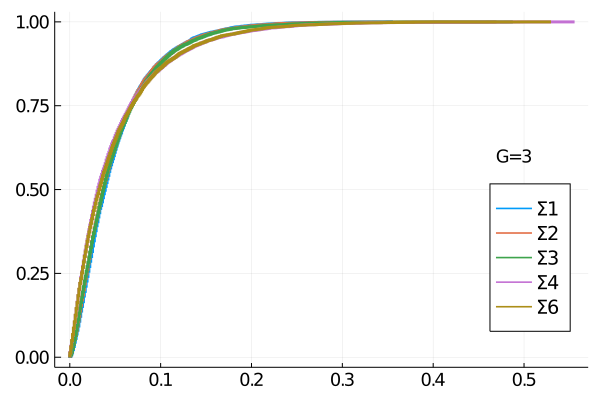
\includegraphics[scale=0.35]{Plots/HO_diffSigmVers2_5MatG3.png}
    \caption{Empirical distribution of the test statistics in Equation~\ref{eq:BFensblPL} under the NULL hypothesis of common mean vector and common covariance matrix across groups.}
    \label{fig:BFh0}
\end{figure}
We formalize that empirical result \textcolor{red}{later on} in the section~\ref{sec:theori}. %Provided the NULL distribution our test statistic $\widetilde{\boldpsi}^{0}$, the decision is made as follows:
%Here $\widetilde{\boldpsi}^{0}_{\alpha}$ denotes the upper $\alpha$ percentile of the NULL distribution.
We also show that the proposed tests are unbiased and their power converges to $1$ with increasing sample size under a sequence of local alternatives (see section~\ref{sec:theori}).  

\subsection{Choices of $m$, $\tau^{*}_{ij}$, and $\ugamma^{*}_{ij}$} \label{sec:testmtaugam}
In this section, we will use $\tau^{*}_{ij}$ to simply refer to $\tau^{PL}_{ij}$ or $\tau^{PR}_{ij}$ depending on what BF we are referring to. Similarly, we will use $\ugamma^{*}_{ij}$ to refer to either $\tau^{PL}_{ij}$ or $\tau^{PR}_{ij}$. 
We obtain values for $m$, $\tau^{*}_{ij}$, and $\ugamma^{*}$ for both $BF^{PL}_{10}$ or $BF^{PR}_{10}$ using the idea of restricted most powerful Bayesian test (RMPBT) proposed by \citealp{GoddardJohnson,Goddard}. To find the RMPBT, we would like to choose the parameters of the prior distribution under the alternative so to maximize the probability of rejecting the NULL under all possible parameters of the data generating model. Namely, for a Bayes Factor in favor of the alternative computed as in Equations~\ref{eq:BFmax},\ref{eq:BFmaxij} for testing our hypothesis for the pair of group $(i,j)$, we will select $\tau^{*}_{ij}$ so that for a given evidence threshold $\ugamma^{*}_{ij} > 0$ and any other $\tau^{*}_{ij,1}$ ($\tau^{*}_{ij,1} \neq \tau^{*}_{ij}$) associated with a second alternative, we have
$$Pr\{BF^{*}_{10}(\tau^{*}_{ij}) \geq  \ugamma^{*}_{ij}\} \geq Pr\{BF^{*}_{20}(\tau^{*}_{ij,1}) \geq \ugamma^{*}_{ij} \},$$
for two different choices of the prior parameters under alternative 1 and alternative 2.
This is equivalent to choosing $\tau^{*}_{ij}$ so that $Pr\{f^{*}_{max} > f^{*}_{max,\;0}(\tau^{*}_{ij},\ugamma^{*}_{ij})\}$ is maximized; which occurs when $f^{*}_{max,\;0}(\tau^{*}_{ij},\ugamma^{*}_{ij})$ is minimized over all possible values of $\tau^{*}_{ij}$ and $\ugamma^{*}_{ij}$. Thus, $f^{PL}_{max,\;0}(\tau^{PL}_{ij},\ugamma^{PL}_{ij}) =\frac{1+\eta_{ij}}{\eta_{ij}} \left\{ \frac{(N - m -G+1)C^{PL}_{ij}}{m(1 - C^{PL}_{ij})} \right\}$, where $C^{PL}_{ij} = \frac{1+\eta_{ij}}{\eta_{ij}}\left\{ 1 - \{\ugamma(1+\eta_{ij})^{m/2} \}^{-2/(N-1)}  \right\}$, $\eta_{ij} = n_{0,ij}/\tau$ (for Bayes Factor in ~\ref{eq:BFmax}) and $f^{PR}_{max,\;0}(\tau^{PR}_{ij},\ugamma^{PR}_{ij}) =\frac{1+\eta_{ij}}{\eta_{ij}} \left\{ \frac{(n_i+n_j - m -G+1)C^{PR}_{ij}}{m(1 - C^{PR}_{ij})} \right\}$ with $C^{PR}_{ij} = \frac{1+\eta_{ij}}{\eta_{ij}}\left\{ 1 - \{\ugamma(1+\eta_{ij})^{m/2} \}^{-2/(n_i+n_j-1)} \right\}$ and $\eta_{ij} = n_{0,ij}/\tau$ (for Bayes Factor in \ref{eq:BFmaxij}). 
Recalling that the statistics $f^{PL}_{ij} \stackrel{id}{\sim} \uF_{m, N - m- (G-1)} $ and $f^{PR}_{ij} \stackrel{id}{\sim} \uF_{m, n_i+n_j - m- 1}$ respectively when $H_0$ is true, we can select $f^{PR}_{max,\;0}$ and $f^{PL}_{max,\;0}$ so that our test has the same size as an equivalent frequentist test. Namely, for a significance level $\alpha$, we will select $f^{PL}_{max,\;0}(\tau^{PL}_{ij},\ugamma^{PL}_{ij})$ and $f^{PR}_{max,\;0}(\tau^{PR}_{ij},\ugamma^{PR}_{ij})$ so that 
$Pr\{f^{PL}_{max} > f^{PL}_{max,\;0}(\tau^{PL}_{ij},\ugamma^{PL}_{ij}, \alpha)\} = \alpha$ and $Pr\{f^{PR}_{max} > f^{PR}_{max,\;0}(\tau^{PR}_{ij},\ugamma^{PR}_{ij}, \alpha)\} = \alpha$ when $H_{0}$ is true respectively. However, obtaining the upper $\alpha$ percentile of the distributions of $f^{PL}_{max}$ and $f^{PR}_{max}$ is a difficult task. Using a monte carlo step would lead to a significant increase in computation. Under the assumption of common group covariance matrices when $H_0$ is true, we have that: 
\be
 f^{PL}_{max,\;0}(\tau^{PL}_{ij},\ugamma^{PL}_{ij}, \alpha) &\approx& \uF_{m, N -m -(G-1)}\{(1 - \alpha)^{1/|\mathcal{P}|}\}, \nonumber\\
 f^{PR}_{max,\;0}(\tau^{PR}_{ij},\ugamma^{PR}_{ij}, \alpha) &\approx& \underset{(i,j)\; \in\; %\mathcal{P}}{\mathrm{argmin}}\; \uF_{m, n_{i}+n_{j} -m -1}(\alpha^{1/|\mathcal{P}|}), \nonumber
 \mathcal{P}}{\mathrm{argmax}}\; \uF_{m, n_{i}+n_{j} -m -1}\{ (1 -\alpha)^{1/|\mathcal{P}|}\}, \nonumber
 \ee
where $\uF_{a, b}(\theta)$ denotes the upper $\theta$ percentile of an $\uF$ distribution with $a$ and $b$ degrees-of-freedom. This approximation seem to work well for small values of $\alpha$ which we will tend to be concerned with. We plot the exact and the estimated quantile for $f^{PL}_{max,\;0}$ and $f^{PR}_{max,\;0}$ with the case of independence added for comparison (see Figure \ref{fig:fig2}).

% 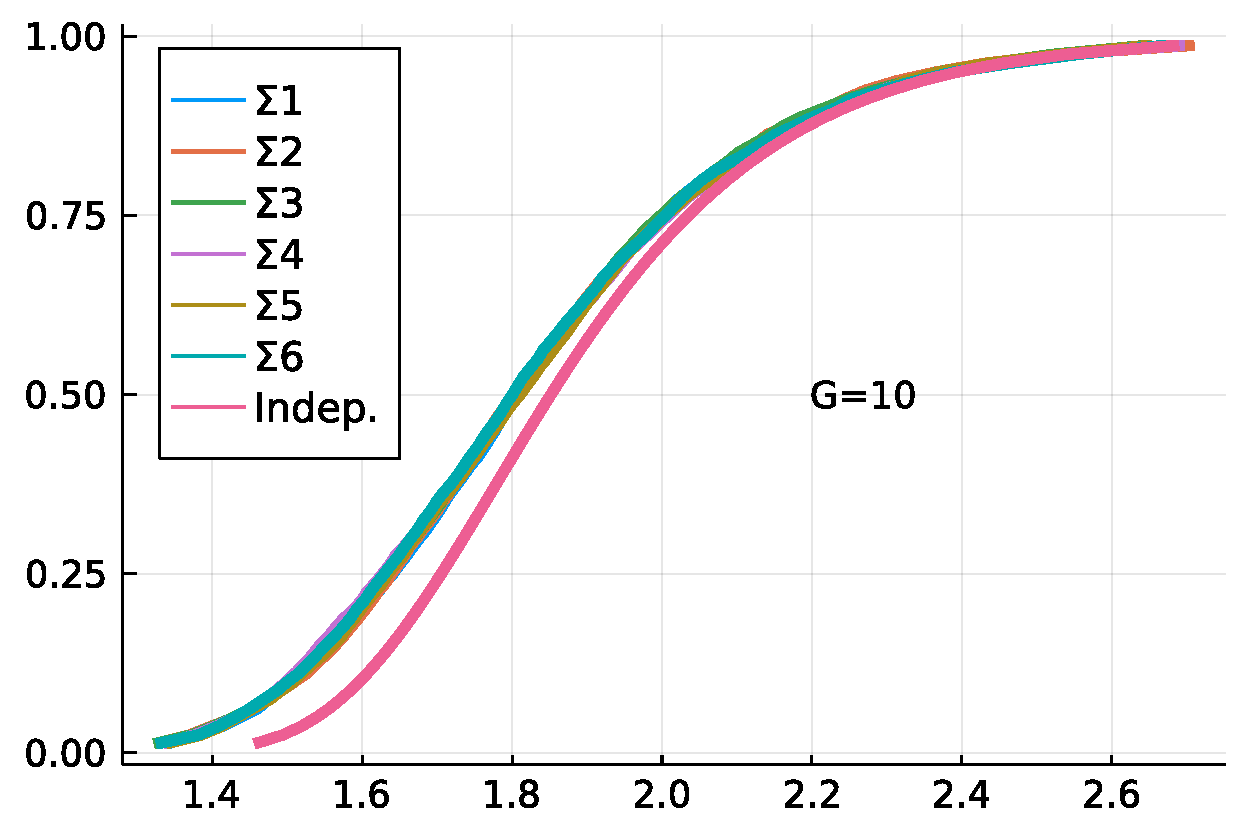
\includegraphics[scale=.5]{Plots/DistFunc_Plot_of F_statBayF_and_F_indep_G_10.pdf}
% 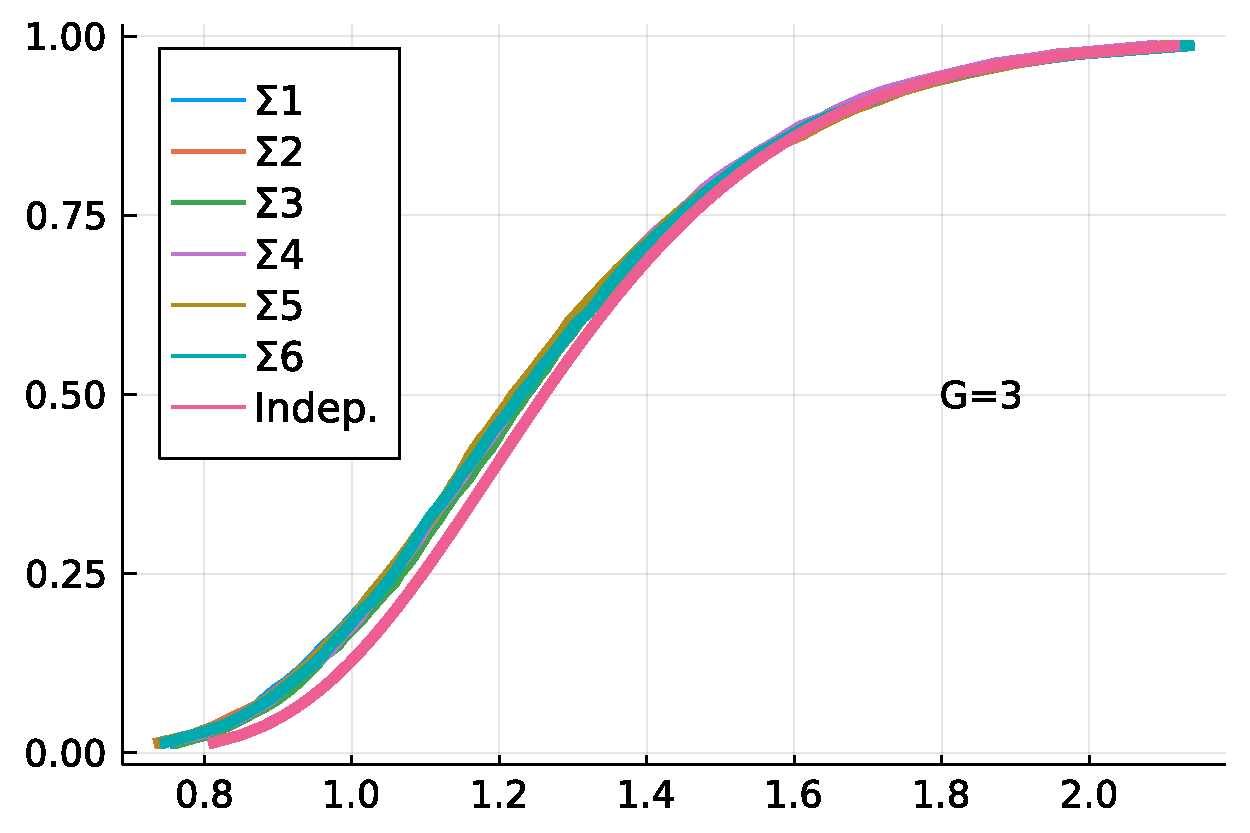
\includegraphics[scale=.5]{Plots/DistFunc_Plot_of F_statBayF_and_F_indep_G_3.pdf}


\begin{figure}
%\begin{subfigure}%{0.3\textwidth}
  \centering
\subfloat[10 groups (45 pairs) ]{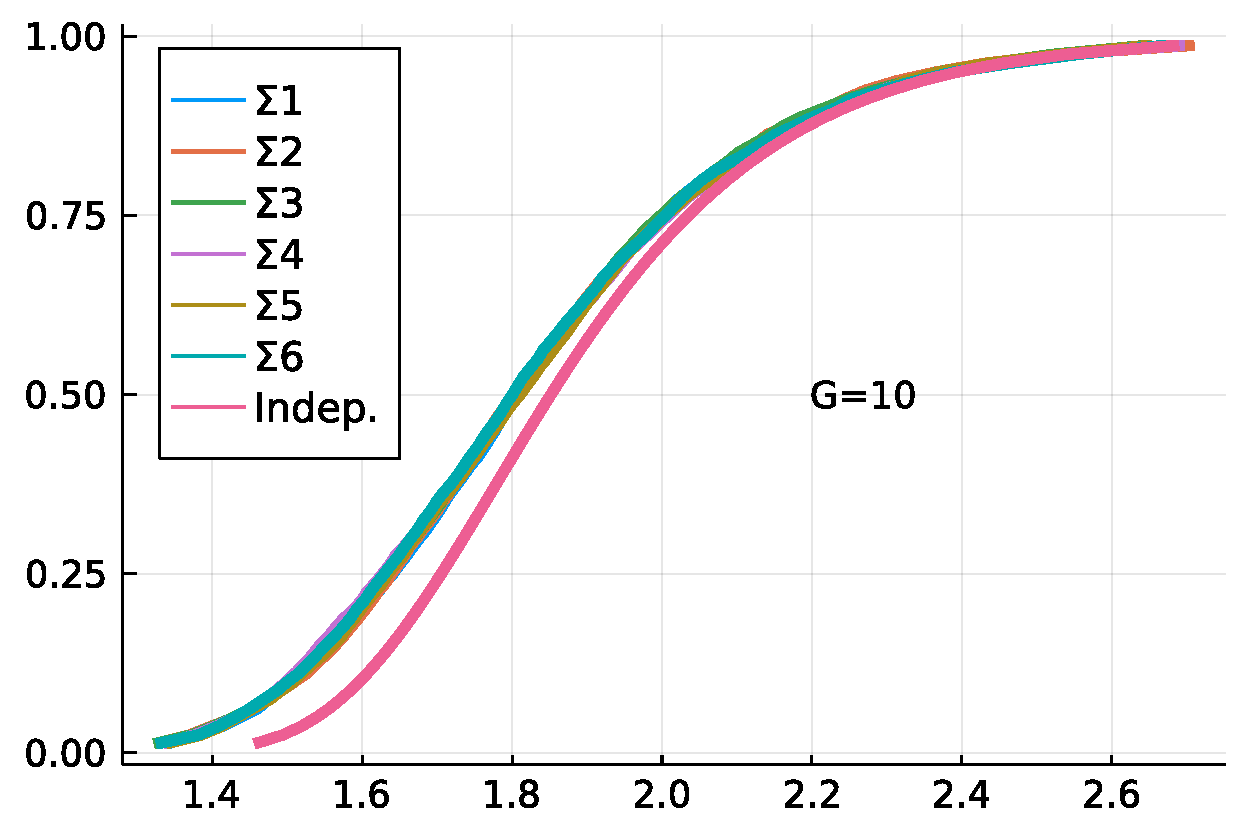
\includegraphics[scale=0.35]{Plots/DistFunc_Plot_of F_statBayF_and_F_indep_G_10.pdf}}
%   \caption{1a}
%   \label{fig:sfig1}
% \end{subfigure}%
% \begin{subfigure}%{0.3\textwidth}
%   \centering
\subfloat[3 groups (3  pairs )]{ 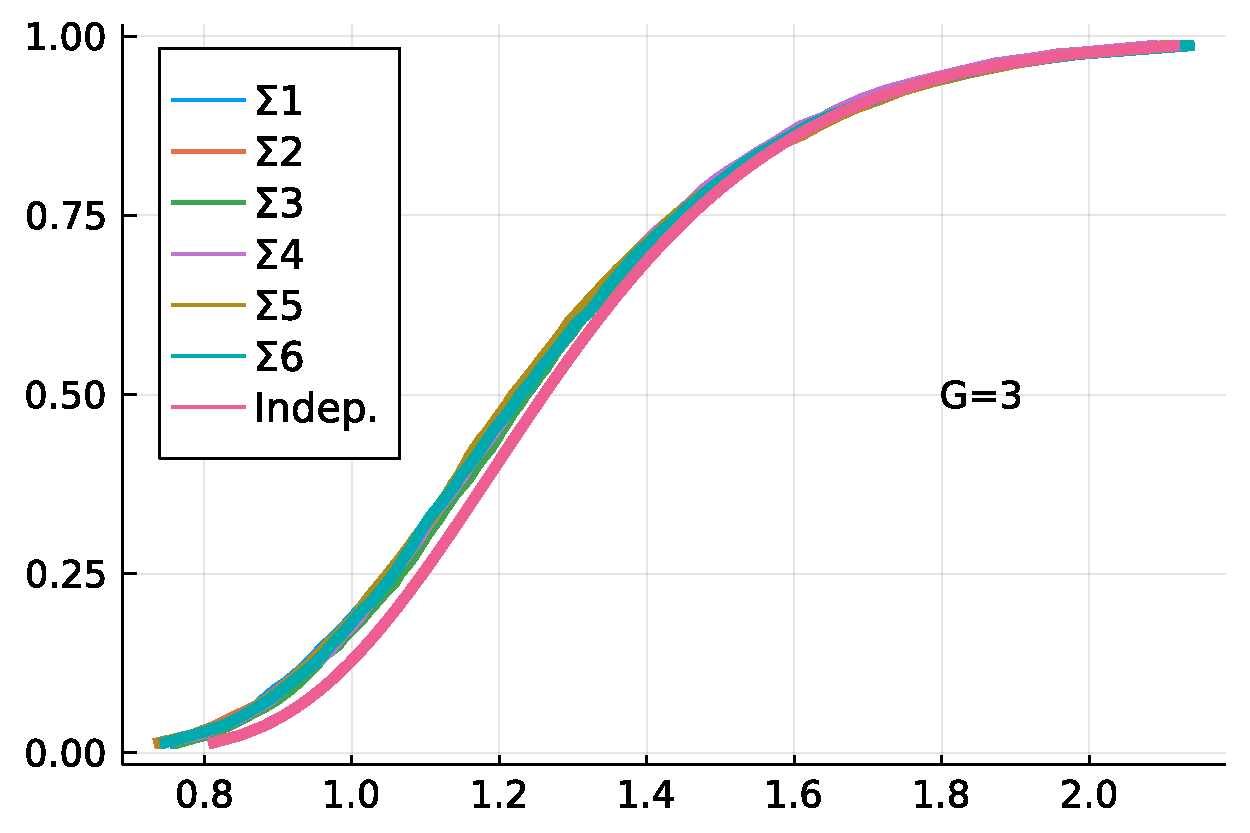
\includegraphics[scale=0.35]{Plots/DistFunc_Plot_of F_statBayF_and_F_indep_G_3.pdf}}
%  \caption{1b}
  \label{fig:fig2}
%\end{subfigure}
\caption{Plots of the empirical distribution of the maximum of identically but correlated $F$ distributed random variables assuming various covariance structure. We also add the case where these $F$ random variables are independent.}
\label{fig:fmaxquant}
\end{figure}

%for all $1 \leq i < j \leq G$ have a marginal $F$ distribution but a complex joint distribution, then we have that for a chosen value of $\alpha$ if $f_{max,\;0}(\tau, \ugamma)$ and $f_{max,\;0}(\tau_{ij},\ugamma)$ are the upper $\alpha$ percentile of the distribution of $f^{PL}_{max}$ and $f^{RP}_{max}$ respectively, then $F_{m, N-m-(G-1)}(\alpha) \leq f^{PL}_{max, \;0}(\tau. \ugamma)$, for the BF in (\ref{eq:BFmax}).  
We can use that fact to obtain an approximate value of $m$ in both cases as:
\be
 \underset{m\; \in\; (1, \min\{n_1, \cdots,n_{G}\})-2}{\mathrm{arg\max}}\; F_{m, N -m -(G-1)}\{1-(1 - \alpha)^{1/|\mathcal{P}|}\}\;\; \mbox{or}\;\; \underset{m}{\mathrm{\min}} \left\{m:\forall\;(i,j) \in\mathcal{P}\;,  \underset{m\; \in \;(1, n_i+n_{j}-2)}{\mathrm{arg\min}}\; F_{m, n_i+n_j -m -1}\{1 - (1 - \alpha)^{1/|\mathcal{P}|}\} \right\}, \label{eq:mval} 
 \ee
for the BF in (\ref{eq:BFmax}) and (\ref{eq:BFmaxij}) respectively; $F_{a, b}(\theta)$ is the upper $\theta \in (0, 0.5)$ percentile of a $F$ distribution with $a$ and $b$ degrees of freedom. We discuss the choice of $\alpha$ shortly.
Next, given $n_1,n_2, \cdots, n_{G}$ and $m$, we can reliably approximate the upper quantiles of $f^{PL}_{max}$ and $f^{PR}_{max}$ under the assumption of common covariance matrix using quantiles of a $\uF$ distribution providing significant savings in computation time (see Figure~\ref{fig:fmaxquant}). Next we obtain, $\tau$, for the pair that yield the maximum $f^{PL}_{max}$ and $f^{PR}_{max}$, which we assume is the pair $(i, j)$.
\be
\tau^{PL}_{ij} = \frac{n_{0,ij}}{\uF_{m, N -m -(G-1)}\{1-(1-\alpha)^{1/|\mathcal{P}|}\} - 1}\; \mbox{and}\; \tau^{PR}_{ij} = \frac{n_{0,ij}}{\left[\underset{(i,j)\; \in\; \mathcal{P}}{\mathrm{argmin}}\; \uF_{m, n_{i}+n_{j} -m -1}\{1-(1-\alpha)^{1/|\mathcal{P}|}\}\right] - 1} , \label{eq:tau0}
\ee
for a significance level $\alpha$;  $1/n_{0,ij} = 1/n_{i} + 1/n_{j}$. %and $\tau^{PL}(n)$ and $\tau^{PR}(n)$ are the values of $\tau$ for the Bayes Factor $BF^{PL}$ and $BF^{PR}$ respectively. %It is c made clear that these values depend on the sample sizes $n_1, \cdots, n_{G}$.  
%Recall $f^{max,0}(\alpha)$ denotes the upper $\alpha$ percentile of a null distribution of $f^{max}$. 
%The choice the $f^{max,0}(\alpha)$ allows us to easily compare our proposed test with a non-Bayesian competitor using a chosen significance level $\alpha$.
%Given $\tau_{}$ and $m$, we can compute the appropriate threshold so our test has a size comparable to that of a frequentist test. 
Subsequently, we obtain the threshold for each Bayes factor Equations for $f^{PL}_{max,\;0}$ and $f^{PR}_{max,\;0}$ respectively as
\be
\ugamma^{PL}_{ij} &=& \left\{ 1 + \eta^{PL}_{ij}\right\}^{-m/2}\left\{ 1 - \frac{\eta^{PL}_{ij}}{1 + \eta^{PL}_{ij}} C^{PL}_{ij} \right\}^{-(N -1)/2} \nonumber \\
\ugamma^{PR}_{ij} &=& \left\{ 1 + \eta^{PR}_{i_1j_1}\right\}^{-m/2}\left\{ 1 - \frac{\eta^{PR}_{i_1j_1}}{1 + \eta^{PR}_{ij}} C^{PR}_{ij} \right\}^{-(n_i+n_j -1)/2} \nonumber
\ee
where $\ugamma^{PF}_{ij}$ and $\ugamma^{PR}_{ij}$ denotes the evidence threshold values respectively for $\text{BF}_{10}^{PL}$ and $\text{BF}^{PR}_{10}$; $\eta^{PL}_{ij} = n_{0,ij}/ \tau^{PL}_{ij}$, and $\eta^{PR}_{ij} = n_{0,ij}/ \tau^{PR}_{ij}$.
and 
\be
\frac{C^{PL}_{ij}}{1 -C^{PL}_{ij}} &=& \frac{ \eta^{PL}_{ij} m}{(1+ \eta^{PL}_{ij})(N - m -(G-1)}f^{PL}_{max,\;0}(\alpha) \nonumber \\
\frac{C^{PR}_{i_1 j_1}}{1 - C^{PR}_{i_1j_1}} &=& \frac{ \eta^{PR}_{i_1 j_1} m}{(1+ \eta^{PR}_{i_1 j_1})(n_{i_1} +n_{j_1} - m -1)}f^{PR}_{max,\;0}(\alpha). \nonumber 
\ee
%We note here that quantities such as $m$ (dimension of the random projection) are computed once for all, but $(\tau^{PL}_{ij}, \tau^{PR}_{ij})$, $(\eta^{PL}_{ij}, \eta^{PR}_{ij})$, $(\ugamma^{PL}_{ij}, \ugamma^{PR}_{ij})$ are computed only for pairs associated with the maximum $f^{PL}_{ij}$ and $f^{PR}_{ij}$ respectively. 
We note both statistics could result in different pairs although here we use the same indices for both test statistics. 

%$\ugamma = \left\{ 1 + \eta_{ij}\right\}^{-m/2}\left\{ 1 - \frac{\eta_{ij}}{1 + \eta_{ij}} C_{ij} \right\}^{-(N -1)/2}$ (for Bayes Factor in \ref{eq:BFmax}) and  %\label{eq:gamma}
%$\gamma_{ij,\alpha} = \left\{ 1 + \eta_{ij}\right\}^{-m/2}\left\{ 1 - \frac{\eta_{ij}}{1 + \eta_{ij}} C_{ij} \right\}^{-(n_i+n_j -1)/2}$ (for Bayes Factor in \ref{eq:BFmaxij}).
Finally, the RP matrices are chosen orthogonal matrices so that for a given RP matrix $\Phi \in \mathbb{R}^{p \times m}$,  $\Phi\trans\Phi = \uI_{m}$. We use the sparse and dense version of the RP matrices proposed by \cite{srivastava2014raptt}. Additionally, the normalization step can be completely skipped based on the results of the QR factorization of a matrix (see \citealp{zoh2018powerful} for more details).
%Each cases of the test statistics considered, the data depending quanty is a $f^{max}$ an $\uF$ statistics.

%First note that for each pair $(i<j) \in \{1, \cdots, p\}$, $f_{i,j}  = \frac{N-m-1)}{(N-2)m} n_{0,ij} (\overline{\uX}_i - \overline{\uX}_j)\trans \uS_{p}^{-1}(\overline{\uX}_i - \overline{\uX}_j) \sim \uF_{m, N-m-(G-1)}$ (marginally). Although the $f_{ij}$ are identically distributed, they are not independent. In fact the distribution of $f_{max}$ is complicated to derive but can simply be approximated under the NULL using a Monte Carlo approach. The simulation will need to be run for multiple values of $m$ which can reveal too expensive. We adopt an approximate approach and obtain $m$ almost as if we were performing a two-sample approach  using the definition of restricted most powerful Bayesian test (RMPBT) approach proposed by \cite{GoddardJohnson,Goddard}. First note that
%Namely, we choose the value of m as
%$$ m = \arg\max_{m} \uF_{m, N-m-(G-1)}(\theta), $$
%where $uF_{\alpha,\beta}(u)$ is the upper $u$ quantile of the $\uF$ distribution with $m$ and $N-m-(G-1)$ degrees-of-freedom. Subsequently, given the value of $m$, we obtain $\gamma$ as
%$$\log(\gamma) =  -.5m\log(1+\tau^{\star}) - .5(N-1)\log\left(1 - \frac{\tau^{\star}}{1 + \tau^{\star}}C_0 \right),$$
%where $C_0 = \frac{mf^{max}_{\theta}}{m f^{max}_{\theta} + N-m-(G-1)}$; $f^{max}_{\theta}$ is the upper $\theta$ quantile of the null distribution of $f^{max}$; $\tau^{\star} = f^{max}_{\theta} -1$. Note for we simply approximate the (NULL) distribution of  $f^{max}$ using a Monte Carlo approach given values of $n_1, n_2, \cdots, n_{G}$ and $m$.

\section{Theoretical justifications and Simulation Results} \label{sec:theori}
Here we adopt a slightly different notation to make clear that the quantities we are referring to are dependent on the sample sizes $n_1, \cdots, n_{G}$. Also, we have $n_{\min} = \min\{n_1,\cdots, n_{G}\}$, $n_{\max} = \max\{n_1,\cdots, n_{G}\}$; $n = \sum^{G}_{g=1}n_g$; $n_{ij} = n_i + n_j$ and $n_{ij,\min} = \min_{(i,j) \in \mathcal{P}} n_{ij}$. 

\subsection{Theoretical Justifications} 
We assume the following conditions.
\begin{description}
  \item[Assumption 1] $n_g /\sum_{g=1}^{G}n_g \rightarrow \theta_1 \in (0, 1)$
  \item[Assumption 2] $G / n_{min} \rightarrow 0$ as $\min\{ n_1, \cdots, n_G \} \rightarrow \infty$ (G is fixed as a function of $n_{\min}$)
  \item[Assumption 3] $n_{\max}/p \rightarrow \theta_2 \in (0, 1)$ 
%  \item[Assumption 4] We denote as $m_n$, $\tau^{\star}_{ij,n}$, and $\gamma^{\star}_{ij,n}$ the values of $m$, $\tau^{\star}_{ij}$ and $\gamma^{\star}_{ij}$ we derived in session~\ref{sec:testmtaugam}. Further, we assume that $m_n/n \rightarrow \theta \in(0, 1)$ so that $m_n n_{0,ij}/\tau^{*}_{ij,n} \rightarrow \infty$ as $n_{\min} \rightarrow \infty$. These conditions are satisfied by our construction (\citealp[see Appendix C of][]{zoh2018powerful}).  
\end{description}

\subsubsection{Consistency of $BF_{10}^{PL}$}
\begin{theorem}\label{Thrm1}
Suppose that $X_{ig} = \umu_i + \uepsilon_{ig}$, where $\uepsilon_{ig} \sim \MVN_{p}(\bzero, \uSigma)$, for $g = 1, \cdots, G$ independent groups and $p >> \max\{n_1, \cdots, n_{G}\}$, where $n_1, \cdots, n_{G}$ are the respective sample sizes. %Suppose $1 \leq m  \leq \min\{n_1, \cdots, n_{G}\}$ and $n_{min} = \min\{n_1, \cdots, n_{G}\}$. Then,  %\sum^{G}_{g=1}n_g$. %Let's $BF^{PL}_{max} = \max\{BF^{PL}_{12}, \cdots, BF^{PL}_{(G-1)G}\}$, where $BF^{PL}_{ij}$ is the BF based on the group $i$ and $j$ data. As $\min\{n_1, \cdots, n_{G}\} \rightarrow \infty$,
\begin{enumerate}
    \item If $m \in (1, n - G)$ and $\tau^{PL}_{ij}$, $\forall (i,j) \in \mathcal{P}$ are pairs, then $\log(BF^{*}_{10}) \rightarrow -\infty$ under $H_0$ and $\log(BF^{PL}_{10}) \rightarrow \infty$ under $H_1$ as $n_{min} \rightarrow \infty$. {\color{blue}I guess the condition $m/n\to \theta\in (0, 1)$ is required in part (1)? Also, it seems that $\tau_{ij}^{PL}$ should be fixed here?}
    \item If 
    % $1 \leq m_n \leq n - G$ so that $m_n/n \rightarrow \theta \in (0, 1)$
    {\color{blue}$m_n$
    and $\tau^{PL}_{ij}$ are selected} according to our construction in section~\ref{sec:testmtaugam}, then $\log(BF^{PL}_{10}) = \mathcal{O}_{p}(1)$ under $H_0$ and $\log(BF^{PL}_{10}) \rightarrow \infty$ under a sequence of local alternative $H_{1,n}$ as $n_{min} \rightarrow \infty$.
\end{enumerate}
\end{theorem}



\begin{proof}[\textbf{\upshape Proof:}]
Our proof uses similar argument to that of \citep{zoh2018powerful}.
\begin{description}
\item[Part(1)]
For $1 < m < n - G$ and $n = \sum^{G}_{g}n_g$, we integrate out the parameters with respect to the conjugate priors to obtain the Bayes Factor in favor of the alternative as
\be
BF^{PL}_{10, ij}(\uPhi) &=&\left(1 + \eta^{PL}_{ij} \right)^{-m/2} \left\{ 1 - \frac{\eta^{PL}_{ij}}{(1 + \eta^{PL}_{ij})}\frac{ m f_{max}^{PL}}{ m f_{\max}^{PL}  + n - m - (G-1)} \right\}^{-(n-1)/2} \nonumber,
\ee
where
\bse
f_{ij}^{PL}  = \frac{n - m - (G-1)}{(n-G)m} n_{0,ij}(\overline{\uX}_i - \overline{\uX}_j)\trans \uPhi(\uPhi\trans \uS\uPhi )^{-1}\uPhi\trans (\overline{\uX}_i - \overline{\uX}_j)
\ese
%and $$f_{max}^{PL} = \arg\max_{(ij) \in \mathcal{P}} f^{PL}{_{ij} $$
and $$ \uS = \frac{1}{n - G} \sum^{G}_{g=1}(n_g -1)\uS_{g}\; \text{and} \;\; \uS_g = \frac{1}{n_g - 1}\sum^{n_g}_{i=1}(\uX_{ig} - \overline{\uX}_{g})(\uX_{ig} - \overline{\uX}_{g})\trans.$$
Recall that $1/n_{0,ij} = 1/n_i + 1/n_j$, $\eta^{PL}_{ij} = n_{0,ij}/\tau^{PL}_{0,ij}$, and $n_{\min} = \min\{n_1, \cdots, n_G\}$.
Since $\tau^{PL}_{ij}$ is fixed, $\eta^{PL}_{ij} \rightarrow \infty$ as $n_{\min} \to \infty$.
For a randomly chosen projection matrix $\uPhi$, under $H_{0}$, $f^{PL}_{ij}  \sim F_{m, n-m-(G-1)}$ with $m$ and $n - m -(G-1)$ degrees of freedom.
Thus, $f^{PL}_{ij} = O_{p}(1)$ and $f^{PL}_{\max} = \arg\max_{(i,j) \in \mathcal{P}}\{ f_{ij}^{PL}\}$.
Also, from well-known properties of the $F$ distribution, we have that
\bse
U_{ij} = \frac{m f_{ij}^{\star}/(n-m-(G-1) )}{\{m f_{ij}^{\star}/(n-m- (G-1) ) + 1\}} = \nonumber \\
  \frac{m f_{ij}^{\star}}{( m f_{ij}^{\star} +n-m- (G-1))} \sim \Beta\{m/2, (n-m-(G-1))/2 \},
\ese
for each $(i,j)$ with $1 \leq i, j \leq G$, where $\Beta(a, b)$ denotes a Beta distribution.
Therefore, $\{\eta^{PL}_{ij}/(1 + \eta^{PL}_{ij})\} U_{ij} = O_{p}(1)$.
Hence, $\log\left\{ 1 -  \eta^{PL}_{ij} U_{ij}/(1 + \eta^{PL}_{ij}) \right\} = O_{p}(1)$ as $n_{\min} \to \infty$. We then get
\bse
-\frac{m}{2n}\log(1 + \eta^{PL}_{ij}) -\frac{(n-1)}{2n}\log\left\{ 1 -  \eta^{PL}_{ij} U_{ij}/(1 + \eta_{ij}^{PL}) \right\} \xrightarrow[]{p} -\infty,
\ese
since $\log(1 + \eta^{PL}_{ij}) \rightarrow \infty$ as $n_{\min} \rightarrow \infty$ and $\lim_{n_{\min} \rightarrow \infty} m/n = \theta \in (0, 1)$.
We conclude that $\log\{BF^{PL}_{10,ij}(\uPhi)\} \xrightarrow[]{p} -\infty$ under the null hypothesis for all $1 \leq i < j \leq G$.
Hence $\log\{BF^{PL}_{10,ij}(\uPhi)\} \xrightarrow[]{p} -\infty$. This result hold for any $(i,j) \in \mathcal{P}$ and we conclude $\log\{BF^{PL}_{10}(\uPhi)\} \xrightarrow[]{p} -\infty$. {\color{blue}This may be related to a previous question: What is the relation between $BF_{10}^{PL}$ and $BF_{10,ij}^{PL}$?}

Under the alternative, $\umu_{i} \neq \umu_{j}$ and $\udelta_{ij} \sim \uN_{p}({\bf 0}, \uSigma /\tau^{PL}_{ij})$.
Then, $f_{ij}^{PL} \mid   \lambda_{ij} \sim F_{m, n-m-(G-1)}(\lambda_{ij})$
with non-centrality $\lambda_{ij} = n_{0,ij}\udelta_{ij}\trans\uPhi(\uPhi\trans \uSigma \uPhi)^{-1}\uPhi\trans \udelta_{ij}$.
Since $\udelta_{ij} \sim \uN_{p}({\bf 0}, \uSigma /\tau_{ij})$, $\lambda_{ij} \sim n_{0,ij}\chi_{m}^{2}/\tau_{ij}$,
where $\chi_{m}^{2}$ denotes a $\chi^{2}$ distribution with m degrees of freedom. The non-centrality parameter depends on $n$ through $n_{0,ij}$.
It can be shown that the unconditional distribution of $f_{ij}^{PL} /(1 + \eta^{PL}_{ij}) \sim F_{m, n-m-(G-1)}$ \citep[see for reference][page 704]{johnson2005bayes}.
If we denote $f_{0,ij}^{PL} =  f_{ij}^{PL} /(1 + \eta^{PL}_{ij})$, we have $f^{PL}_{0,ij} = O_{p}(1)$, and $mf_{0,ij}^{PL}/n = O_{p}(1)$, as $n_{\min} \rightarrow \infty$.
We have that
\be
\frac{\eta^{PL}_{ij} U_{ij}}{(1+\eta^{PL}_{ij})} = \frac{ m f_{ij}^{0}\eta^{PL}_{ij}}{m f_{ij}^{0}(1+\eta^{PL}_{ij})+n-m-(G-1)} \nonumber
\ee
From the above equation, we get
\be
-\log\left\{ 1 - \frac{\eta^{PL}_{ij} U_{ij}}{(1+\eta^{PL}_{ij})} \right \} &=& \log\left\{ \frac{mf_{0,ij}^{PL}(1+\eta^{PL}_{ij})/(n-m-(G-1)) + 1}{\{mf_{0,ij}^{PL}/(n-m-(G-1))\} +1 }\right\}. \nonumber
\ee
Since $f_{ij}^{0} = O_{p}(1)$, and $m/(n-m-1)$ converges, we have
\bse
 -\log\left\{ 1 - \frac{\eta^{PL}_{ij} U_{ij}}{(1+\eta^{PL}_{ij})} \right \} \xrightarrow[]{p} \infty.
\ese
Since this is true for all $(i,j)$ where $\umu_i \neq \umu_j$ with $1 \leq i < j \leq G$, we conclude that $\log\left\{BF^{PL}_{10,ij}(\uPhi) \right \} \xrightarrow[]{p} \infty$, under the alternative hypothesis. Hence $\log\left\{BF^{PL}_{10}(\uPhi) \right \} \xrightarrow[]{p} \infty$ under the alternative. 

\item[Part(2)] First let's show that $m_n/n \rightarrow a \in (0, 1)$. 
We have that for a chosen $G$ and samples sizes $n_1, \cdots, n_{G}$,  $F_{\alpha, m, n-m_n-(G-1)}$ is convex over the range of possible values of $m_n \in (1, n-G)$. For large values of $m_n$ and $n - m_n$, we have $F_{\alpha, m_n, n-m_n-(G-1)}$ is convex suggesting that $m_n$ and $n-m_n$ diverge. {\color{blue}It seems unclear to me why $F_{\alpha, m, n - m - (G - 1)}$ being convex w.r.t. $m$ implies that $m$ and $n - m$ diverge. However, I came up with a somewhat more rigorous proof and provide it below. The proof requires an additional condition that $\alpha < 0.25$. ($\alpha < 0.25$ may not be the weakest condition but in practice it can be mostly satisfied.)}

{\color{blue}
We prove that $m_n\to\infty$ by contradiction, and the proof of the claim that $n - m_n\to\infty$ is similar by taking the reciprocal of the $F$ distribution. Namely, there exists a subsequence $(n_k)_{k = 1}^\infty$ such that $m_{n_k}\to \bar{m}$ for some fixed $\bar{m}\in\mathbb{N}_+$ as $k\to\infty$. Since $m_n$'s are integers, it follows that $m_{n_k} = \bar{m}$ for sufficiently large $k$. By the properties of the $F$ distribution, we have $F_{m_{n_k}, n_k - m_{n_k} - (G - 1)} \overset{\mathcal{L}}{\to} \chi^2_{\bar{m}}/\bar{m}$, where $\chi^2_{\bar{m}}$ is the chi-squared distribution with degree of freedom $\bar{m}$. By the convergence of the quantile function, this implies that $F_{\alpha, m_{n_k}, n_k - m_{n_k} - (G - 1)}\to \chi_{\alpha,\bar{m}}^2/\bar{m}$, where $\chi_{\alpha,\bar{m}}^2$ is the upper $\alpha$ quantile of $\chi_{\bar{m}}^2$. Since $\alpha < 0.25$, by the Berry-Esseen bound, we have that $\chi_{\alpha,\bar{m}}^2/\bar{m} > 1$ for any fixed $\bar{m}$, implying that $F_{\alpha, m_{n_k}, n_k - m_{n_k} - (G - 1)} > 1$ for sufficiently large $k$. On the other hand, if $(m_n^*)_{n = 1}^\infty$ is a sequence with $m^*_n/\sqrt{n}\to 1$ as $n\to\infty$, then by the central limit theorem and the weak law of large numbers, $\sqrt{m_n^*}(F_{m_n^*,n - m_n^* - (G - 1)} - 1)\overset{\mathcal{L}}{\to}\mathrm{N}(0, 2)$, thereby implying that $F_{\alpha, m_n^*, n - m_n^* - (G - 1)}\to 1$ by the convergence of the quantile. This further shows that $F_{\alpha, m_{n_k}^*, n_k - m_{n_k}^* - (G - 1)} < F_{\alpha, m_{n_k}, n_k - m_{n_k} - (G - 1)}$ for sufficiently large $k$. Hence, $m_{n_k}$ cannot be the minimizer of $F_{\alpha, m, n_k - m - (G - 1)}$ w.r.t. $m$ because $m_{n_k}^*$ gives a smaller value of the quantile. This contradicts with the definition of $m_{n_k} = \arg\min_mF_{\alpha, m, n_k - m - (G - 1)}$, and thus, we have $\liminf_{n\to\infty}m_n = \infty$.
}

We have that for large $m_n$ and $n-m_n$, then $F_{\alpha, m_n, n-m_n-(G-1)} \approx \mu_n + \sigma_n\Phi^{-1}(\alpha)$, where $\mu_n = \frac{n-m_n-(G-1)}{n-m_n-(G-1) - 2} > 1$ and $\sigma^2_n = \frac{2(n-m_n-(G-1))^2 (n-(G-1)-2)}{m_n(n-m_n-(G-1))(n-m_n-(G-1)-2)^2}$; $\Phi^{-1}(\alpha)$ is the upper $\alpha$ percentile of the standard normal distribution. Thus the quantile of F distribution is at it minimum if when $\sigma^2_n$ is minimum. Thus, using the result from \cite{zoh2018powerful}, we have that $m_n \approx n/2$ thus $m_n/n \rightarrow 1/2$ as $n_{\min} \rightarrow \infty$. 

$\eta^{PL}_{ij} = n_{0,ij}/\tau^{PR}_{ij} = F_{1-(1-\alpha)^{1/|\mathcal{P}|},m_n, n-m_n-(G-1)} - 1 \rightarrow 0$, since $\mu_m \rightarrow 1$ and $\sigma^2_n = \mathcal{O}(1/m_n)$ and thus  $F_{1-(1-\alpha)^{1/|\mathcal{P}|},m_n, n-m_n-(G-1)} \rightarrow 1$ converges to $1$ as $n_{\min} \rightarrow \infty$. 
We see that $F_{1-(1-\alpha)^{1/|\mathcal{P}|}, m_n, n-m_n-(G-1)} -1 $ converges to 0 at a slower rate than $1/\sqrt{n}$. We conclude that $n\eta^{PR}_{ij} \rightarrow \infty$ and $m_{n}\eta^{PR}_{ij} \rightarrow \infty$ as $n_{\min} \rightarrow \infty.$
%We now assume that $\eta^{PL}_{ij} \rightarrow 0$ and $m_n \eta^{PL}_{ij} \rightarrow \infty$. 

We have the following expression for the $\log$ Bayes factor. 
\be
 \log\{BF^{PL}_{10,ij}(\uPhi)\} =\frac{n}{2}\left( 1 - \frac{m_n}{n}\right)\log\left(1 + \eta^{PL}_{ij} \right) - \frac{n}{2}\log\left\{ 1 + \eta^{PL}_{ij}(1-U_{ij}) \right \} +\frac{1}{2}\log \left\{1 - \frac{\eta^{PL}_{ij} U_{ij}}{1+\eta^{PL}_{ij}}\right\},  \nonumber
\ee
where $U_{ij} \sim Beta\left\{ m_n/2,  (n - m_n -(G-1))/2 \right\}$ under $H_0$ for each $1 \leq i < j \leq G$.
For large $n$ (large $n_{\min}$), none of the terms with $n$ dominates and their difference converges.
The distribution $ \log\{BF^{PL}_{10, ij}(\uPhi) \}$ then depends on that of $U_{ij}$, which is bounded in probability when the null hypothesis is true.
Therefore, under $H_0$, $\log\{BF^{PL}_{10, ij}(\uPhi) \} = \mathcal{O}_{p}(1)$ and we conclude $\log\{BF^{PL}_{10}(\uPhi) \} = \mathcal{O}_{p}(1)$ for each $(i,j) \in \mathcal{P}$.

Under $H_{1,n}$ and $\umu_i \neq \umu_j$ for a $(i,j) \in \mathcal{P}$, again we have
\be
\log\{BF^{PL}_{10,ij}(\uPhi) \} = -\frac{m_n}{2}\log(1 + \eta^{PL}_{ij}) - \frac{(n-1)}{2}\log\left\{ 1 - \frac{\eta^{PL}_{ij} U_{ij}}{1 + \eta^{PL}_{ij}} \right\}, \nonumber
\ee
where $U_{ij} \xrightarrow[]{p} 1$ with $f^{PL}_{ij}\xrightarrow[]{p} \infty$.
{\color{blue}It is not quite clear to me why $U_{ij} \overset{p}{\to} 1$ but I guess $U_{ij} = O_p(1)$ should be enough because $\eta_{ij}^{PL}\to 0$. }
Since $\log(1 + \eta^{PL}_{ij})\{ (n-1)/2 - m_n/2\} \rightarrow \infty$, we conclude that $\log\{BF^{PL}_{10,ij}(\uPhi) \} \xrightarrow[]{p} \infty $ for $(i,j) \in \mathcal{P}$ where $\umu_i \neq \umu_j$. Hence $\log\{BF^{PL}_{10}(\uPhi) \} \xrightarrow[]{p} \infty $.
\end{description}
\end{proof}

\subsubsection{Consistency of $BF_{10}^{PR}$}
\begin{theorem}\label{Thrm2}
Suppose that $X_{ig} = \umu_i + \uepsilon_{ig}$, where $\uepsilon_{ig} \sim \MVN_{p}(\bzero, \uSigma)$, for $g = 1, \cdots, G$ independent groups and $p >> \max\{n_1, \cdots, n_{G}\}$, where $n_1, \cdots, n_{G}$ are the respective sample sizes. %Suppose $1 \leq m  \leq \min\{n_1, \cdots, n_{G}\}$ and $n_{min} = \min\{n_1, \cdots, n_{G}\}$. Then,  %\sum^{G}_{g=1}n_g$. %Let's $BF^{PL}_{max} = \max\{BF^{PL}_{12}, \cdots, BF^{PL}_{(G-1)G}\}$, where $BF^{PL}_{ij}$ is the BF based on the group $i$ and $j$ data. As $\min\{n_1, \cdots, n_{G}\} \rightarrow \infty$,
\begin{enumerate}
    \item If $m \in (1,  n_{ij,\min} - 2)$ and $\tau^{PR}_{ij}$, $\forall (i,j) \in \mathcal{P}$ pairs, then $\log(BF^{PR}_{10}) \rightarrow -\infty$ under $H_0$ and $\log(BF^{PR}_{10}) \rightarrow \infty$ under $H_1$ as $n_{min} \rightarrow \infty$. 
    \item If $m_n \in (1,  n_{ij,\min} -2)$ so that $m_n/n \rightarrow a \in (0, 1)$ and $\tau^{PR}_{ij}$ according to our construction in section~\ref{sec:testmtaugam}, then $\log(BF^{PR}_{10}) = \mathcal{O}_{p}(1)$ under $H_0$ and $\log(BF^{PL}_{10}) \rightarrow \infty$ under a sequence of local alternative $H_{1,n}$ as $n_{min} \rightarrow \infty$.
\end{enumerate}
\end{theorem}
The proof of Theorem \ref{Thrm2} is very similar to Theorem~\ref{Thrm1} and is omitted here. 
\begin{comment}

\begin{proof}[\textbf{\upshape Proof:}]
\begin{description}
\item[Part(1)]
For $1 < m < \min\{ n_1, \cdots, n_{G} \}$ and $n = n_i + n_j$, we integrate out the parameters with respect to the conjugate priors to obtain the Bayes Factor in favor of the alternative as
\be
BF^{PR}_{10,ij}(\uPhi) &=&\left(1 + \eta_{ij} \right)^{-m/2} \left\{ 1 -  \frac{ m f_{ij}^{\star} \eta_{ij}/(1 + \eta_{ij}) }{ m f_{ij}^{\star}  + n_{ij} - m - 1} \right\}^{-(n_{ij}-1)/2} \nonumber,
\ee
where
\bse
f_{ij}^{\star}  = \frac{n_{ij} - m - 1}{(n_{ij}-2)m} n_{0,ij}(\overline{\uX}_i - \overline{\uX}_j)\trans \uPhi(\uPhi \uS_{ij}\uPhi\trans )^{-1}\uPhi\trans (\overline{\uX}_{i} - \overline{\uX}_{j}).
\ese
where $$ \uS_{ij} = \frac{1}{n_{ij} - 2} \sum_{g=(i,j)}(n_g -1)\uS_{g}\; \text{and} \;\; \uS_g = \frac{1}{n_g - 1}\sum^{n_g}_{l=1}(\uX_lg - \overline{\uX}_{g})(\uX_lg - \overline{\uX}_{g})\trans.$$
Recall that $1/n_{0,ij} = 1/n_i + 1/n_j$, $\eta_{ij} = n_{0,ij}/\tau_{0,ij}$, and $n_{\min} = \min\{n_i, n_j\}$.
Since $\tau_{0,ij}$ is fixed, $\eta_{ij} \rightarrow \infty$ as $n_{\min} \to \infty$.
For a randomly chosen $\uPhi$, under $H_{0}$, $f_{ij}^{\star}  \sim F_{m, n_{ij}-m-1}$ with $m$ and $n_{ij} - m -1$ degrees of freedom.
Thus, $f_{ij}^{\star} = O_{p}(1)$ and $f^{max}_{ij} = \max_{ij}\{ f^{\star}_{ij}\}$ for all $1 \leq i, j \leq G$.
Also, from well-known properties of the $F$ distribution, we have that
\bse
U_{ij} = \frac{m f_{ij}^{\star}/(n_{ij}-m-1 )}{\{m f_{ij}^{\star}/(n_{ij} - m - 1 )\}} = \nonumber \\
  \frac{m f_{ij}^{\star}}{( m f_{ij}^{\star} + n_{ij} - m-1)} \sim \Beta\{m/2, (n_{ij}-m-1)/2 \},
\ese
for each $ij$ with $1 \leq i, j \leq G$, where $\Beta(a, b)$ denotes a Beta distribution.
Therefore, $\{\eta_{ij}/(1 + \eta_{ij})\} U_{ij} = O_{p}(1)$.
Hence, $\log\left\{ 1 -  \eta_{ij} U_{ij}/(1 + \eta_{ij}) \right\} = O_{p}(1)$ as $n_{\min} \to \infty$. We then get
\bse
-\frac{m}{2n_{ij}}\log(1 + \eta_{ij}) -\frac{(n_{ij}-1)}{2n_{ij}}\log\left\{ 1 -  \eta_{ij} U_{ij}/(1 + \eta_{ij}) \right\} \xrightarrow[]{p} -\infty,
\ese
since $\log(1 + \eta_{ij}) \rightarrow \infty$ as $n_{\min} \rightarrow \infty$ and $\lim_{n_{\min} \rightarrow \infty} m/n_{ij} = \theta \in (0, 1)$.
We conclude that $\log\{BF^{PR}_{ij}(\uPhi)\} \xrightarrow[]{p} -\infty$ under the null hypothesis for all $1 \leq i < j \leq G$.
Hence $\log\{BF^{PR}_{10}(\uPhi)\} \xrightarrow[]{p} -\infty$.

Under the alternative, $\umu_{i} \neq \umu_{j}$ and $\udelta_{ij} \sim \uN_{p}({\bf 0}, \uSigma /\tau_{0})$.
Then, $f_{ij}^{\star} \mid   \lambda_{ij} \sim F_{m, n_{ij}-m-1}(\lambda_{ij})$
with non-centrality $\lambda_{ij} = n_{0,ij}\udelta_{ij}\trans\uPhi(\uPhi\trans \uSigma \uPhi)^{-1}\uPhi\trans \udelta_{ij}$.
Since $\udelta_{ij} \sim \uN_{p}({\bf 0}, \uSigma /\tau_{0})$, $\lambda \sim n_{0,ij}\chi_{m}^{2}/\tau_{0}$,
where $\chi_{m}^{2}$ denotes a $\chi^{2}$ distribution with m degrees of freedom. The non-centrality parameter depends on $n_{ij}$ through $n_{0,ij}$.
We can show that the unconditional distribution of $f_{ij}^{\star} /(1 + \eta_{ij}) \sim F_{m, n_{ij}-m-1}$ \citep[see][page 704]{johnson2005bayes}.
If we denote $f_{ij}^{0} =  f_{ij}^{\star} /(1 + \eta_{ij})$, we have $f_{ij}^{0} = O_{p}(1)$, and $mf_{ij}^{0}/n_{ij} = O_{p}(1)$, as $n_{\min} \rightarrow \infty$.
We have that
\be
\frac{\eta_{ij} U_{ij}}{(1+\eta_{ij})} = \frac{ m f_{ij}^{0}\eta_{ij}}{m f_{ij}^{0}(1+\eta_{ij})+n_{ij}-m-1} \nonumber
\ee
From the above equation, we get
\be
-\log\left\{ 1 - \frac{\eta_{ij} U_{ij}}{(1+\eta_{ij})} \right \} &=& \log\left\{ \frac{mf_{ij}^{0}(1+\eta_{ij})/(n_{ij}-m-1) + 1}{\{mf_{ij}^{0}/(n-m-1)\} +1 }\right\}. \nonumber
\ee
Since $f_{ij}^{0} = O_{p}(1)$, and $m/(n_{ij}-m-1)$ converges, we have
\bse
 -\log\left\{ 1 - \frac{\eta_{ij} U_{ij}}{(1+\eta_{ij})} \right \} \xrightarrow[]{p} \infty.
\ese
Since this is true for all $(i,j)$ with $\umu_i \neq \umu_j$ with $1 \leq i < j \leq G$,  we conclude that $\log\left\{BF^{PR}_{10}(\uPhi) \right \} \xrightarrow[]{p} \infty$, under the alternative hypothesis.

\item[Part(2)]
We now assume that $\eta_{ij} \rightarrow 0$ and $m_n \eta_{ij} \rightarrow \infty$. We have
\be
 \log\{BF^{PR}_{10}(\uPhi)\} =\frac{n_{ij}}{2}\left( 1 - \frac{m_n}{n_{ij}}\right)\log\left(1 + \eta_{ij} \right) - \frac{n_{ij}}{2}\log\left\{ 1 + \eta_{ij}(1-U_{ij}) \right \} +\frac{1}{2}\log \left\{1 - \frac{\eta_{ij} U_{ij}}{1+\eta_{ij}}\right\},  \nonumber
\ee
where $U_{ij} \sim Beta\left\{ m/2,  (n_{ij} - m_n -(G-1))/2 \right\}$ under $H_0$ for each $1 \leq i < j \leq G$.
For large $n_{ij}$, none of the terms with $n_{ij}$ dominates and their difference converges.
The distribution of $\log\{BF^{PR}_{10}(\uPhi) \}$ then depends on that of $U$, which is bounded in probability.
Therefore, under $H_0$, $\log\{BF^{PR}_{10, ij}(\uPhi) \} = \mathcal{O}_{p}(1)$ and we conclude $\log\{BF^{PL}_{10}(\uPhi) \} = O_{p}(1)$ for all $1 \leq i < j \leq G$.

Under $H_{1,n}$, again we have
\be
\log\{BF^{PR}_{10,ij}(\uPhi) \} = -\frac{m}{2}\log(1 + \eta) - \frac{(n_{ij}-1)}{2}\log\left\{ 1 - \frac{\eta U}{1 + \eta} \right\}, \nonumber
\ee
where $U_{ij} \xrightarrow[]{p} 1$ with $f_{ij}^{*}\xrightarrow[]{p} \infty$.
Since $\log(1 + \eta_{ij})\{ (n_{ij}-1)/2 - m_n/2\} \rightarrow \infty$, we conclude that $\log\{BF^{PR}_{10,ij}(\uPhi) \} \xrightarrow[]{p} \infty $ for $(i,j)$ where $\umu_i \neq \umu_j$. Hence $\log\{BF^{PR}_{10}(\uPhi) \} \xrightarrow[]{p} \infty $
\end{description}
\end{proof}
\end{comment}

\refmark{\bf Remarks:}
We make the following remarks about the both Bayes factors. 
\begin{enumerate}
    \item Theorems~\ref{Thrm1} and ~\ref{Thrm2} show that both Bayes factors we constructed have the same behavior as the usual Bayes Factor, i.e consistent for a chosen projection dimension $m$, alternative $\tau_{ij}$, and evidence threshold $\gamma_{ij}$ all independent of the groups sizes. 
    \item Theorems~\ref{Thrm1} and ~\ref{Thrm2} show that under our prescribed construction for $m_n$, $\tau^{\star}_{ij}$, $\gamma^{\star}_{ij}$ as in section~\ref{Thrm2}, both Bayes factors we constructed are bounded in probability under the null hypothesis. However, under the sequence of alternative $H_{1,n}$ associated with $\tau^{*}_{ij}$ (dependent on sample sizes), the Bayes Factor converges to $+\infty$.
\end{enumerate}



\subsubsection{Power of the ensemble test}
\begin{theorem}
Suppose the assumptions of Theorems~\ref{Thrm1} and ~\ref{Thrm2} hold.
Given a collection $\uPhi_1, \cdots, \uPhi_N$ of independent random projections matrices,
where $\uPhi_{i}\trans\uPhi_{i} = \uI$ for all $i = 1, \cdots, N$ ($N$ potential large), then $\lim_{n_{\min} \rightarrow \infty} Pr\{\widetilde{\boldpsi}^{\star}(N) > \widetilde{\boldpsi}^{\star}_{0,\alpha}\}  = 1$ under the sequence $H_{1,n}$ of alternatives.

Where $\widetilde{\boldpsi}^{\star}(N)\;(\widetilde{\boldpsi}^{\star}_{0,\alpha})$ denotes either the $\widetilde{\boldpsi}^{PL}(N)\; (\widetilde{\boldpsi}^{PL}_{0,\alpha})$ or $\widetilde{\boldpsi}^{PR}(N)\;(\widetilde{\boldpsi}^{PR}_{0,\alpha})$. 
%\begin{description}
%\item[part(a)] Under $H_0$, $E\{\boldpsi}(N)\}  = \alpha$
%\item[part(b)] 
%\end{description}
\end{theorem}
\begin{proof}[\textbf{\upshape Proof:}]
The proof is similar to that of \citealp{zoh2018powerful} and the will use the $(\star)$ to denote either tests.  
The power of our test is $Pr\{ \widetilde{\psi}^{\star}(N) > \widetilde{\psi}^{\star}_{0,\alpha}\mid  H_{1,n}\}$.
Henceforth, we make it explicit that $\widetilde{\psi}^{\star}_{0,\alpha}$ depends on $(n_1, \cdots ,n_G)$ and write $\widetilde{\psi}^{\star}_{0,\alpha}(n_1, \cdots, n_G)$ instead.

Given $n_1, \cdots, n_G$ and $\alpha$, we choose $\widetilde{\psi}^{\star}_{0,\alpha}(n_1, \cdots, n_G)$ so that $Pr\{\widetilde{\psi}^{\star}(N) > \widetilde{\psi}^{\star}_{0, \alpha}(n_1, \cdots,n_G)\mid  H_{0}\}  = \alpha$.
Since $ 0 < \widetilde{\psi}^{\star}_{0,\alpha}(n_1, \cdots,n_G) < 1$, for $0 < \alpha < 1$, we have that $Pr\{ \sum^{N}_{i=1}\widetilde{\psi}^{\star}(\uPhi_i) \geq 0 \mid H_{1,n} \} \geq Pr\{ \sum^{N}_{i=1}\widetilde{\psi}^{\star}(\uPhi_i) > N\widetilde{\psi}^{\star}_{0,\alpha}(n_1, \cdots ,n_G) \mid H_{1,n} \} \geq Pr\{ \sum^{N}_{i=1}\widetilde{\psi}^{\star}(\uPhi_i) \geq N \mid H_{1,n} \}$.

We have that $Pr\{\widetilde{\psi}^{\star}(\uPhi_i) =1 \mid H_{1,n}\} \rightarrow 1$ as $n_{\min} \rightarrow \infty$, under the alternative for $i = 1, \cdots, N$. So, $Pr\{ \sum^{N}_{i=1}\widetilde{\psi}^{\star}(\uPhi_i) \geq 0 \mid H_{1,n} \} = 1 - \prod_{i=1}^{N}Pr\{\widetilde{\psi}^{\star}(\uPhi_i) = 0 \mid H_{1,n} \} \rightarrow 1$.
Additionally, $Pr\{ \sum^{N}_{i=1}\widetilde{\psi}^{\star}(\uPhi_i) \geq N \mid H_{1,n} \} = Pr\{ \sum^{N}_{i=1}\widetilde{\psi}^{\star}(\uPhi_i) = N \mid H_{1,n} \} = \prod_{i=1}^{N}Pr\{\widetilde{\psi}^{\star}(\uPhi_i) = 1 \mid H_{1,n}\} \rightarrow 1$ for fixed $N$ as $n_{\min} \rightarrow \infty$. We conclude that $Pr\{ \widetilde{\psi}^{\star}(N) \geq \widetilde{\psi}^{\star}_{0, \alpha}\mid  H_{1,n}\} \rightarrow 1$ as $n_{\min} \rightarrow \infty.$
\end{proof}

\subsection{Simulation}

\subsubsection{Simulation Study design}
We designed a simulation study aimed at investigating the power of the tests proposed in section~\ref{sec:test}
with respect to the proportion of true elements of $\umu$ that are actually zero (for none all zero vectors) for various choices of covariance matrices and different proportions of non zeros vectors.
Broadly, we consider two settings for our simulation. In each case, we have two conditions for each choice of the covariance matrix. 
In the first condition, we assume $p = 200$, $G=3, 5$ and $n_g = 50\;\forall\; g =  1, \cdots, G$. Using the approach described above (Section~\ref{sec:test}), we find $m = 43$ for the test based on $BF^{PR}_{10}$ for both $G=3,5$. However, for the test based on $BF_{10}^{PR}$, we get $m = 65$ and $m = 111$ when $G=3$ and $G=5$ respectively. 
In the second condition, $p = 1000$, $G=3, 5$ and $n_g = 70$, $\forall\; 1 \leq g \leq G$ and we get $m = 62$ for the test based on $BF^{PR}_{10}$. For the test based on $BF^{PL}_{10}$, we get $m = 105, 175$ respectively for $G=3$ and $G=5$. We denote by $p_0$ the proportion of entries of the vector $\udelta$ that are exactly zero. We choose $p_0 = 0.5, .75, .80, 0.95, 0.99, 1.00$ (NULL hypothesis).
In each setting, the values of $\tau^{\star}_{ij}$ and $\gamma^{\star}_{ij}$ are chosen according to our discussion in Section~\ref{sec:testmtaugam} for both tests. We consider two types of random projections matrices, $\uPhi_{1}$(full matrix)  and $\uPhi_2$ (sparse matrix) as described in \citealp{srivastava2014raptt,zoh2018powerful}. Finally, we assume $\alpha = 0.05$.

In \textbf{case 1}, only the last group $G$ has a non-zero mean vector $\umu_G$. But all the others groups have vector mean zero. In \textbf{case 2}, only the last group $G$ has a zero vector mean $\umu_{G}$ and a fixed proportions of the entries of the other group mean vectors are selected to be non-zeros.  
We consider the following choices of covariance matrix $\uSigma=(\sigma_{ij})$.
\begin{enumerate}
  \item $\uSigma_{1} = \uI_{p \times p} $ is the identity matrix.
  \item $\uSigma_{2} $ is block diagonal matrix, with block $\uB = 0.85\uI_{25 \times 25} + 0.15\uJ_{25 \times 25}$. $\uJ$ denotes a matrix with 1 in all of its entries.
  \item $\uSigma_{3}$ is a diagonal matrix where the $20\%$ of the entries of the diagonal elements are $\sigma^2_j = 0.2p/j$ for $j = 1, \cdots, 0.2p$ and the remaining $\sigma^2_j = 1$ for $j > 0.2p$.
  \item $\uSigma$ is an AR(1) covariance matrix with $\sigma_{ij}=\sigma^2\rho^{|i - j|}\bone(|i-j| < 2)$. We chose $\sigma^2 = 1$ and $\rho = 0.4$.
  \item $\uSigma_{5}$ is an AR(1) covariance matrix with $\sigma_{ij}=\sigma^2\rho^{|i - j|}$. We chose $\sigma^2 = 1$ and $\rho = 0.6$.
%  \item $\uSigma_5$ is an ARIMA(1,1) covariance matrix with $\sigma_{ij}=\sigma^{2}\gamma^{1\{|i-j|>0\}}\rho^{|i-j| 1\{|i-j| \geq 2\}}$.
  \item $\uSigma_6 = \uD^{1/2}\left\{ \uI_K \bigotimes (.2\uI_2 + \uJ_{2}0.8) \right\}\uD^{1/2}$, where $\diag(\uD)=(d_{1}, \cdots, d_{p})\trans$ and $d_{1}, \cdots, d_{p} \sim \text{Uniform}(1, 3)$ and $K = p/2$; $\uI$ is the identity matrix and $\uJ$ a matrix of all ones.
  %We chose $\sigma^{2} = 1$, $\gamma = 0.5$, $\rho = 0.9$.
\end{enumerate}
For each case, we also consider two possible alternatives. We simulate the non-all zeros mean vectors as follow
\begin{enumerate} %[label=(\alph*)]
 \item[{\bf Alt.2:}]  $\umu_g \sim \uN_{p}(\bf{1}, \uI)$, set $p_0$ randomly selected elements to zero, and re-scale $\umu_g$ so that $\umu_g \trans\uSigma ^{-1}  \umu_g = 2$ 
 \item[{\bf Alt.1:}] $\umu_g \sim \uN_{p}(\bf{1}, \uI)$ and set $p_0$ of its elements to zero and re-scale $\umu_g$ so that $\frac{||\umu_{g}||^{2}}{\sqrt{\trace\left( \uSigma ^{2}\right)}} = 0.1$.
\end{enumerate}
The two alternatives described above were also considered by \citet{srivastava2014raptt,zoh2018powerful}.

\subsubsection{Simulation Results}
We first look at the performance of the both tests ($BF^{PL}_{10}$ and $BF^{PR}_{10}$) in term of their empirical power for simulation {\bf case 1} under alternative 1 (See Tables~\ref{tab:table1},~\ref{tab:table2}). 
Overall both tests tended to have an empirical type 1 error estimate around $5\%$; although in  some case the estimated type error seems slight inflated for the case of complex covariance matrices. 
We note a significant difference between both tests in term of the estimated empirical power. 
For the same setting, now looking at {\bf case 2}, we observations made in {\bf case1} still hold (see Tables S.1 ans S.2 from the Supplemental Material), except we observe a higher estimated power for the test on $BF^{PR}_{10}$. Recall that in case 2, only the last group non-zero mean vector. 
The test based on the paired groups($BF^{PR}_{10}$) performs much better when compared to the test based on the pooled covariance for data simulated under the alternative 1. 
Note that the data were simulated under the common covariance model. 
However, for data simulated under Alternative 2, again assuming common group covariance matrices, we see that both the tests based on pooled covariance ($BF^{PL}_{10}$) and the test based on the pairwise groups ($BF^{PR}_{10}$) performs very similarly. Although the test based on $BF^{PL}_{10}$ tended to have slightly higher power and estimated Type 1 error near $0.05$ (see Tables~\ref{tab:table3}~\ref{tab:table4}).

%Alternative 1 and Group 3, case1
%Alternative 1 and Group 3, case1 (Pairwise BF)
\begin{table}[ht]
\centering
\caption{ Empirical estimates of the power for the test based on $BF^{PR}$ when data are simulated as in case (1) and based on the Alternative 1. Note here $\text{cp}$ refers to the true covariance matrix (G = 3). }
%Alternative 1 and Group 3, case1 (Pairwise BF)}
\label{tab:table1}
\resizebox{\columnwidth}{!}{%
\begin{tabular}{|rr|rrrrrr|rrrlll|} \hline
  &&\multicolumn{6}{c|}{ $\uPhi_1$} & \multicolumn{6}{c|}{ $\uPhi_2$} \\ \hline
   & cp &  1 & 0.99 & 0.95 & 0.8 & 0.75 & 0.5 & 1 & 0.99 & 0.95 & 0.8 & 0.75 & 0.5 \\ 
  \hline
    \multirow{6}{*}{\rotatebox[origin=c]{90}{$n=50, p=200$}}
  & 1 &  0.033 & 0.833 & 0.711 & 0.675 & 0.633 & 0.658 &  0.033 & 0.833 & 0.711 & 0.675 & 0.633 & 0.658 \\ 
  & 2 &  0.034 & 0.796 & 0.654 & 0.666 & 0.616 & 0.668 &  0.034 & 0.796 & 0.654 & 0.666 & 0.616 & 0.668 \\ 
    & 3 &  0.038 & 0.780 & 0.643 & 0.610 & 0.586 & 0.589 & 0.038 & 0.780 & 0.643 & 0.610 & 0.586 & 0.589 \\ 
    & 4 &  0.049 & 0.494 & 0.408 & 0.396 & 0.402 & 0.451 &  0.049 & 0.494 & 0.408 & 0.396 & 0.402 & 0.451 \\ 
   & 5 &  0.064 & 0.437 & 0.347 & 0.343 & 0.329 & 0.375 &  0.064 & 0.437 & 0.347 & 0.343 & 0.329 & 0.375 \\ 
    & 6 &  0.073 & 0.283 & 0.235 & 0.224 & 0.217 & 0.237 &  0.073 & 0.283 & 0.235 & 0.224 & 0.217 & 0.237 \\ 
  \cline{3-14} \\
  \cline{3-14}
     \multirow{6}{*}{\rotatebox[origin=c]{90}{$n=70,p=1000$}}&  
     1 & 0.021 & 0.340 & 0.321 & 0.305 & 0.310 & 0.288 &  0.021 & 0.340 & 0.321 & 0.305 & 0.310 & 0.288 \\ 
   & 2 & 0.031 & 0.322 & 0.278 & 0.286 & 0.293 & 0.331 &  0.031 & 0.322 & 0.278 & 0.286 & 0.293 & 0.331 \\ 
    & 3 &  0.062 & 0.292 & 0.262 & 0.237 & 0.237 & 0.233 & 0.062 & 0.292 & 0.262 & 0.237 & 0.237 & 0.233 \\ 
    & 4 &  0.036 & 0.179 & 0.174 & 0.157 & 0.170 & 0.203 & 0.036 & 0.179 & 0.174 & 0.157 & 0.170 & 0.203 \\ 
     & 5 &  0.065 & 0.179 & 0.180 & 0.151 & 0.160 & 0.192 &  0.065 & 0.179 & 0.180 & 0.151 & 0.160 & 0.192 \\ 
   & 6 & 0.047 & 0.143 & 0.126 & 0.104 & 0.119 & 0.134 &  0.047 & 0.143 & 0.126 & 0.104 & 0.119 & 0.134 \\ 
   \hline
\end{tabular}
}
\end{table}

%----- alternative 1 and Group 3
%Alternative 1,  Group=3, case1 (Common Covariance)
\begin{table}[ht]
\centering
\caption{ Empirical estimates of the power for the test based on $BF^{PL}$ when data are simulated as in case (1) and based on the Alternative 1. Note here $\text{cp}$ refers to the true covariance matrix (G = 3). }
\label{tab:table2}
\resizebox{\columnwidth}{!}{%
\begin{tabular}{|rr|rrrrrr|rrrlll|} \hline
 & &\multicolumn{6}{c|}{ $\uPhi_1$} & \multicolumn{6}{c|}{ $\uPhi_2$} \\ \hline
   & cp &  1 & 0.99 & 0.95 & 0.8 & 0.75 & 0.5 & 1 & 0.99 & 0.95 & 0.8 & 0.75 & 0.5 \\ 
  \hline
    \multirow{6}{*}{\rotatebox[origin=c]{90}{$n=50, p=200$}} 
 & 1 &   0.034 & 0.050 & 0.042 & 0.033 & 0.051 & 0.045  & 0.034 & 0.050 & 0.042 & 0.033 & 0.051 & 0.045 \\ 
  & 2 &   0.031 & 0.059 & 0.049 & 0.051 & 0.058 & 0.043  & 0.031 & 0.059 & 0.049 & 0.051 & 0.058 & 0.043 \\ 
 & 3 &   0.038 & 0.039 & 0.037 & 0.035 & 0.042 & 0.044  & 0.038 & 0.039 & 0.037 & 0.035 & 0.042 & 0.044 \\ 
   & 4 &   0.049 & 0.064 & 0.053 & 0.067 & 0.059 & 0.055  & 0.049 & 0.064 & 0.053 & 0.067 & 0.059 & 0.055 \\ 
  & 5 &   0.063 & 0.076 & 0.068 & 0.074 & 0.076 & 0.067  & 0.063 & 0.076 & 0.068 & 0.074 & 0.076 & 0.067 \\ 
  & 6 &   0.056 & 0.066 & 0.065 & 0.064 & 0.072 & 0.065  & 0.056 & 0.066 & 0.065 & 0.064 & 0.072 & 0.065 \\ 
   \cline{3-14} \\
  \cline{3-14}
    \multirow{6}{*}{\rotatebox[origin=c]{90}{$n=70,p=1000$}} 
  & 1 &   0.024 & 0.025 & 0.027 & 0.026 & 0.033 & 0.026  & 0.024 & 0.025 & 0.027 & 0.026 & 0.033 & 0.026 \\ 
  & 2 &   0.051 & 0.040 & 0.043 & 0.036 & 0.044 & 0.039  & 0.051 & 0.040 & 0.043 & 0.036 & 0.044 & 0.039 \\ 
  & 3 &   0.065 & 0.071 & 0.068 & 0.050 & 0.056 & 0.061  & 0.065 & 0.071 & 0.068 & 0.050 & 0.056 & 0.061 \\ 
   & 4 &   0.043 & 0.031 & 0.043 & 0.030 & 0.042 & 0.043  & 0.043 & 0.031 & 0.043 & 0.030 & 0.042 & 0.043 \\ 
   & 5 &   0.065 & 0.069 & 0.063 & 0.066 & 0.070 & 0.071  & 0.065 & 0.069 & 0.063 & 0.066 & 0.070 & 0.071 \\ 
  & 6 &   0.049 & 0.036 & 0.058 & 0.053 & 0.042 & 0.066  & 0.049 & 0.036 & 0.058 & 0.053 & 0.042 & 0.066 \\ 
   \hline
\end{tabular}
}
\end{table}

% latex table generated in R 4.1.0 by xtable 1.8-4 package
% Sat Dec  4 22:38:26 2021
% case1 - Alternative 2 - Group 3 (Pairwise BF)
\begin{table}[ht]
\centering
\caption{ Empirical estimates of the power for the test based on $BF^{PR}$ when data are simulated as in case (1) and based on the Alternative 2. Note here $\text{cp}$ refers to the true covariance matrix (G = 3). }
\label{tab:table3}
\resizebox{\columnwidth}{!}{%
\begin{tabular}{|rr|rrrrrr|rrrlll|} \hline
 & &\multicolumn{6}{c|}{ $\uPhi_1$} & \multicolumn{6}{c|}{ $\uPhi_2$} \\ \hline
   & cp &  1 & 0.99 & 0.95 & 0.8 & 0.75 & 0.5 & 1 & 0.99 & 0.95 & 0.8 & 0.75 & 0.5 \\ 
  \hline
    \multirow{6}{*}{\rotatebox[origin=c]{90}{$n=50, p=200$}} 
 & 1 &  0.033 & 0.570 & 0.450 & 0.429 & 0.408 & 0.408 &  0.033 & 0.570 & 0.450 & 0.429 & 0.408 & 0.408 \\ 
  & 2 & 0.034 & 0.790 & 0.637 & 0.598 & 0.537 & 0.508 & 0.034 & 0.790 & 0.637 & 0.598 & 0.537 & 0.508 \\
  & 3 &  0.038 & 0.989 & 0.997 & 1 & 0.996 & 0.998 &  0.038 & 0.989 & 0.997 & 1 & 0.996 & 0.998 \\ 
 & 4 &  0.049 & 0.716 & 0.603 & 0.563 & 0.518 & 0.518 &  0.049 & 0.716 & 0.603 & 0.563 & 0.518 & 0.518 \\ 
 & 5 & 0.064 & 0.944 & 0.843 & 0.802 & 0.755 & 0.706 &  0.064 & 0.944 & 0.843 & 0.802 & 0.755 & 0.706 \\ 
  & 6 & 0.073 & 0.869 & 0.770 & 0.717 & 0.694 & 0.680 &  0.073 & 0.869 & 0.770 & 0.717 & 0.694 & 0.680 \\ 
    \cline{3-14} \\
  \cline{3-14}
    \multirow{6}{*}{\rotatebox[origin=c]{90}{$n=70,p=1000$}}& 
 1 &  0.021 & 0.704 & 0.655 & 0.628 & 0.635 & 0.606 &  0.021 & 0.704 & 0.655 & 0.628 & 0.635 & 0.606 \\ 
  & 2 &  0.031 & 0.864 & 0.830 & 0.789 & 0.759 & 0.716 &  0.031 & 0.864 & 0.830 & 0.789 & 0.759 & 0.716 \\ 
  & 3 &  0.062 & 1 & 1 & 1 & 1 & 1 &  0.062 & 1 & 1 & 1 & 1 & 1 \\ 
 & 4 &  0.036 & 0.818 & 0.759 & 0.739 & 0.730 & 0.696 &  0.036 & 0.818 & 0.759 & 0.739 & 0.730 & 0.696 \\ 
 & 5 &  0.065 & 0.943 & 0.905 & 0.872 & 0.862 & 0.827 &  0.065 & 0.943 & 0.905 & 0.872 & 0.862 & 0.827 \\ 
 & 6 &  0.047 & 0.899 & 0.859 & 0.823 & 0.818 & 0.794 &  0.047 & 0.899 & 0.859 & 0.823 & 0.818 & 0.794 \\ 
   \hline
\end{tabular}
}
\end{table}

% latex table generated in R 4.1.0 by xtable 1.8-4 package
% Sat Dec  4 23:01:10 2021
%Alternative 2,  Group=3, case1 (Common Covariance BF)
\begin{table}[ht]
\centering
\caption{ Empirical estimates of the power for the test based on $BF^{PL}_{10}$ when data are simulated as in case 1 and based on the Alternative 2. Note here $\text{cp}$ refers to the true covariance matrix (G = 3). }
\label{tab:table4}
\resizebox{\columnwidth}{!}{%
\begin{tabular}{|rr|rrrrrr|rrrlll|} \hline
 & &\multicolumn{6}{c|}{ $\uPhi_1$} & \multicolumn{6}{c|}{ $\uPhi_2$} \\ \hline
 & cp &  1 & 0.99 & 0.95 & 0.8 & 0.75 & 0.5 & 1 & 0.99 & 0.95 & 0.8 & 0.75 & 0.5 \\ 
  \hline
    \multirow{6}{*}{\rotatebox[origin=c]{90}{$n=50, p=200$}} 
  & 1 &  0.034 & 0.564 & 0.450 & 0.438 & 0.437 & 0.427  & 0.034 & 0.564 & 0.450 & 0.438 & 0.437 & 0.427 \\ 
 & 2 &  0.031 & 0.781 & 0.674 & 0.590 & 0.596 & 0.530  & 0.031 & 0.781 & 0.674 & 0.590 & 0.596 & 0.530 \\ 
 & 3 &  0.038 & 0.986 & 0.996 & 1 & 0.997 & 0.999  & 0.038 & 0.986 & 0.996 & 1 & 0.997 & 0.999 \\ 
 & 4 &  0.049 & 0.715 & 0.612 & 0.559 & 0.577 & 0.532  & 0.049 & 0.715 & 0.612 & 0.559 & 0.577 & 0.532 \\ 
 & 5 &  0.063 & 0.944 & 0.868 & 0.803 & 0.788 & 0.733  & 0.063 & 0.944 & 0.868 & 0.803 & 0.788 & 0.733 \\ 
 & 6 &  0.056 & 0.872 & 0.783 & 0.731 & 0.739 & 0.708  & 0.056 & 0.872 & 0.783 & 0.731 & 0.739 & 0.708 \\ 
   \cline{3-14} \\
  \cline{3-14}
    \multirow{6}{*}{\rotatebox[origin=c]{90}{$n=70,p=1000$}}
  & 1 &  0.024 & 0.738 & 0.662 & 0.664 & 0.650 & 0.659  & 0.024 & 0.738 & 0.662 & 0.664 & 0.650 & 0.659 \\ 
  & 2 &  0.051 & 0.894 & 0.817 & 0.811 & 0.812 & 0.775  & 0.051 & 0.894 & 0.817 & 0.811 & 0.812 & 0.775 \\ 
  & 3 &  0.065 & 1 & 1 & 1 & 1 & 1  & 0.065 & 1 & 1 & 1 & 1 & 1 \\ 
  & 4 &  0.043 & 0.839 & 0.772 & 0.764 & 0.776 & 0.748  & 0.043 & 0.839 & 0.772 & 0.764 & 0.776 & 0.748 \\ 
  & 5 &  0.065 & 0.947 & 0.916 & 0.889 & 0.910 & 0.859  & 0.065 & 0.947 & 0.916 & 0.889 & 0.910 & 0.859 \\ 
  & 6 &  0.049 & 0.910 & 0.864 & 0.833 & 0.854 & 0.839  & 0.049 & 0.910 & 0.864 & 0.833 & 0.854 & 0.839 \\ 
   \hline
\end{tabular}
}
\end{table}

We also look at the performance of both tests for the case of $5$ groups (see Tables S.3-S.6 of the Supplemental Material). The observation made for the case of 3 groups also hold for the case of 5.

In the second part of the simulation, we simulate data assuming different covariance matrices between the active group (non-zero) mean vector and the non-active group (all zeros) mean vector. Namely, in {\bf case 1} all groups are assumed to have an identity covariance and the last group $G$ is assumed to have one of the  covariance matrix $\uSigma_k$, for each $k = 1, \cdots, 6$ (see Table~\ref{tab:table5}). 
In {\bf case 2}, however, the active group (Group G) has an identity  covariance matrix and the  non-active groups have the same covariance matrix which is one of the $\uSigma_k$, for each $k = 1, \cdots, 6$. Under these settings, we see that the test statistic based on $BF^{PL}_{10}$ (pooled covariance) is poorly calibrated when the covariance matrices are (very) different. So we do not discuss its estimated power here. We instead focus on the test based on $BF^{PR}_{10}$ (Table~\ref{tab:table6}). The test based on on the $BF^{PR}_{10}$ seems to hold the nominal Type I error for the case small sample size, even though the estimated Type error 1 seems inflated for the covariance matrix very different from the identity matrix.

% latex table generated in R 4.1.0 by xtable 1.8-4 package
% Sat Dec  4 23:19:35 2021
\begin{table}[ht]
\centering
%\caption{Alternative 2,  Group=3, case1 (Pairwise Covariance BF)}
\caption{ Empirical estimates of the power for the test based on $BF^{PR}_{10}$ when data are simulated as in case 2 and based on the Alternative 2. Note here $\text{cp}$ refers to the true covariance matrix (G = 3). }
\label{tab:table5}
\resizebox{\columnwidth}{!}{%
\begin{tabular}{|rr|rrrrrr|rrrlll|} \hline
 & & \multicolumn{6}{c|}{ $\uPhi_1$} & \multicolumn{6}{c|}{ $\uPhi_2$} \\ \hline
  & cp &  1 & 0.99 & 0.95 & 0.8 & 0.75 & 0.5 & 1 & 0.99 & 0.95 & 0.8 & 0.75 & 0.5 \\ 
  \hline
  \multirow{6}{*}{\rotatebox[origin=c]{90}{$n=50, p=200$}}
  & 1 &  0.030 & 0.551 & 0.435 & 0.410 & 0.392 & 0.392 &  0.030 & 0.551 & 0.435 & 0.410 & 0.392 & 0.392 \\ 
  & 2 &  0.033 & 0.745 & 0.608 & 0.562 & 0.504 & 0.505 &  0.033 & 0.745 & 0.608 & 0.562 & 0.504 & 0.505 \\ 
  & 3 &  0.039 & 0.997 & 1 & 1 & 0.999 & 1 &  0.039 & 0.997 & 1 & 1 & 0.999 & 1 \\ 
  & 4 &  0.041 & 0.671 & 0.544 & 0.538 & 0.476 & 0.485 &  0.041 & 0.671 & 0.544 & 0.538 & 0.476 & 0.485 \\ 
  & 5 &  0.053 & 0.845 & 0.738 & 0.700 & 0.651 & 0.631 &  0.053 & 0.845 & 0.738 & 0.700 & 0.651 & 0.631 \\ 
  & 6 &  0.086 & 0.980 & 0.942 & 0.925 & 0.915 & 0.914 &  0.086 & 0.980 & 0.942 & 0.925 & 0.915 & 0.914 \\
    \cline{3-14} \\
  \cline{3-14}
    \multirow{6}{*}{\rotatebox[origin=c]{90}{$n=70,p=1000$}}
  & 1 &  0.024 & 0.621 & 0.554 & 0.539 & 0.526 & 0.509 &  0.024 & 0.621 & 0.554 & 0.539 & 0.526 & 0.509 \\ 
  & 2 &  0.015 & 0.811 & 0.763 & 0.714 & 0.708 & 0.667 &  0.015 & 0.811 & 0.763 & 0.714 & 0.708 & 0.667 \\ 
  & 3 &  0.059 & 1 & 1 & 1 & 1 & 1 &  0.059 & 1 & 1 & 1 & 1 & 1 \\ 
  & 4 &  0.011 & 0.738 & 0.692 & 0.659 & 0.659 & 0.617 &  0.011 & 0.738 & 0.692 & 0.659 & 0.659 & 0.617 \\ 
  & 5 &  0.034 & 0.916 & 0.864 & 0.838 & 0.845 & 0.810 &  0.034 & 0.916 & 0.864 & 0.838 & 0.845 & 0.810 \\ 
  & 6 &  0.087 & 1 & 0.999 & 0.998 & 0.999 & 0.997 &  0.087 & 1 & 0.999 & 0.998 & 0.999 & 0.997 \\ 
  \hline
\end{tabular}
}
\end{table}

%\subsection{Alternative 2,  Group=3, case2 (Pairwise Covariance BF)}
% latex table generated in R 4.1.0 by xtable 1.8-4 package
% Sat Dec  4 23:22:00 2021
\begin{table}[ht]
\centering
%\caption{Alternative 2,  Group=3, case2 (Pairwise Covariance BF)}
\caption{ Empirical estimates of the power for the test based on $BF^{PR}_{10}$ when data are simulated as in case 1 and assuming the Alternative 2. Note here $\text{cp}$ refers to the true covariance matrix (G = 3). Here the data is simulated assuming different covariance matrices. }
\label{tab:table6}
\resizebox{\columnwidth}{!}{%
\begin{tabular}{|rr|rrrrrr|rrrlll|} \hline
 & &\multicolumn{6}{c|}{ $\uPhi_1$} & \multicolumn{6}{c|}{ $\uPhi_2$} \\ \hline
 & cp &  1 & 0.99 & 0.95 & 0.8 & 0.75 & 0.5 & 1 & 0.99 & 0.95 & 0.8 & 0.75 & 0.5 \\ 
  \hline
  \multirow{6}{*}{\rotatebox[origin=c]{90}{$n=50, p=200$}}
  & 1 &   0.030 & 0.921 & 0.866 & 0.782 & 0.781 & 0.712 &  0.030 & 0.921 & 0.866 & 0.782 & 0.781 & 0.712 \\ 
 & 2 &   0.033 & 0.993 & 0.966 & 0.922 & 0.931 & 0.881 &  0.033 & 0.993 & 0.966 & 0.922 & 0.931 & 0.881 \\ 
  & 3    & 0.039 & 1 & 1 & 1 & 1 & 1 &  0.039 & 1 & 1 & 1 & 1 & 1 \\ 
  & 4   & 0.041 & 0.979 & 0.952 & 0.885 & 0.910 & 0.821 &  0.041 & 0.979 & 0.952 & 0.885 & 0.910 & 0.821 \\ 
  & 5   & 0.053 & 1 & 0.995 & 0.992 & 0.986 & 0.970 &  0.053 & 1 & 0.995 & 0.992 & 0.986 & 0.970 \\ 
 & 6 & 0.086 & 1 & 0.997 & 0.994 & 0.994 & 0.983 &  0.086 & 1 & 0.997 & 0.994 & 0.994 & 0.983 \\ 
      \cline{3-14} \\
  \cline{3-14}
    \multirow{6}{*}{\rotatebox[origin=c]{90}{$n=70,p=1000$}}
     & 1   & 0.024 & 0.989 & 0.981 & 0.956 & 0.960 & 0.906 &  0.024 & 0.989 & 0.981 & 0.956 & 0.960 & 0.906 \\
  & 2   & 0.015 & 0.999 & 0.999 & 0.995 & 0.994 & 0.973 &  0.015 & 0.999 & 0.999 & 0.995 & 0.994 & 0.973 \\ 
  & 3    & 0.059 & 1 & 1 & 1 & 1 & 1 &  0.059 & 1 & 1 & 1 & 1 & 1 \\ 
    & 4   & 0.011 & 0.996 & 0.993 & 0.989 & 0.980 & 0.966 &  0.011 & 0.996 & 0.993 & 0.989 & 0.980 & 0.966 \\ 
  & 5   & 0.034 & 1 & 1 & 1 & 1 & 1 &  0.034 & 1 & 1 & 1 & 1 & 1 \\ 
  & 6   & 0.087 & 1 & 1 & 1 & 1 & 1 &  0.087 & 1 & 1 & 1 & 1 & 1 \\ 
  \hline
\end{tabular}
}
\end{table}

\section{Application} \label{sec:Application}
The data set used in our application originated from a head and neck squamous cell carcinoma (HNSCC) study where the profile of $5902$ single cells from 18 patients with oral cavity tumors by single cell RNA-seq are obtained. See \citep{puram2017single} for the detailed description of the study designed. The data set used for our analysis can be downloaded from the Gene expression Omnibus (\textbf{https://www.ncbi.nlm.nih.gov/geo/query/acc.cgi?acc=GSE103322}). Subsequently, each of the $5902$ cells are identified and labelled %(see table for the breakdown).
We would like to know if there is evidence that cell types have different gene expression profile while accounting for the potential dependency between the genes. We frame this problem as a high-dimensional mean vector testing. Under the NULL hypothesis, all cell types have equal or similar mean gene expression profile. Before we can apply our proposed test, we perform a feature reduction step to root out lowly expressed genes. Similar to the approach considered by \cite{puram2017single}, we choose genes with $E_a(i) > 6$, where $E_a(i)=\log2\text{(average(TPM(i)1...k)+1)}$. This results in $p = 2641$ genes selected. We consider the less popular (Tumor free) cell types (3 types): B-cells (n=138),  Macrophage (n=98), and Mast(n=120). To perform our test, we select the dimension of the projections space, according to our discussion above, to be $m = 88$ (for the test based on $BF^{PR}_{10}$) and $m = 161$ for the test based on $BF^{PL}_{10}$, and the evidence threshold is set at $\gamma = 6.340$, and $\alpha = 0.05$. Since our test might be sensible to significant departure of assumption of common covariance, we perform a test comparing covariance matrices (\citealp{ahmad2017location,srivastava2010testing}). Interesting enough, the test proposed by \citealt{ahmad2017location} reject the NULL hypothesis ($p-value < 0.001$). But the covariance test proposed by \cite{srivastava2010testing} does not reject the NULL ($p-value = 0.1878$). 
Finally, applying our test to the data set, we reject the NULL hypothesis with a $p-value < 0.001$ based on the NULL hypothesis of the test statistic in (\ref{eq:BFensbl}) approximated assuming zero mean vectors for each group and a common identity covariance matrix. In all, the test based on Bayes Factor assuming common over all covariance matrix ($BF^{PL}_{10}$) and the test based on pairwise Bayes Factor $(BF^{PR}_{10})$ both yield the same result for the projection matrices $\uPhi_1$ and $\uPhi_2$. 
Our testing procure also provides an automatic way to extract information about all pairwise comparisons since the value of each $f_{ij}$ statistic is retained. A useful summary statistic we can look at is the proportions of $f_{ij}$ statistic that exceeded the threshold of significance across all random projections (see table~\ref{tab:table7a}). We note that the test assuming common covariance across all group $BF^{PL}_{10}$ tended to have a larger proportion of significant test for all pairwise comparisons when compared to its $BF^{PR}_{10}$ counterpart.  

\begin{table}[ht]
\centering
%\caption{Cell type breakdown from \cite{puram2017single}. }
\caption{Proportion of pairwise tests that were declared significant across $1000$ random projections. The results are reported for the both tests $(BF^{PR}_{10}, BF^{PL}_{10})$ .}
\label{tab:table7a}
\begin{tabular}{|rrr|}
  \hline
   & Macrophage & B Cell \\
    Mast & (0.763, 0.943)  & (0.689, 0.819) \\
    Macrophage & - & (0.987, 1.0)  \\
  \hline
\end{tabular}
\end{table}

%   \text{Mat}_{\varphi\text{ to }M} = \kbordermatrix{
%     & Macrophage & B Cell \\
%     Mast & 0.763, 0.943)  & (0.689, 0.819) \\
%     Macrophage & - & (0.987, 1.0)  \\
%   %  B Cell & 0 & 0  \\
%   }
% \]

%$$

%Endothelial(n=260),
% latex table generated in R 4.1.0 by xtable 1.8-4 package
% Tue Nov 30 15:53:17 2021
% \begin{table}[ht]
% \centering
% \caption{Cell type breakdown from \cite{puram2017single}. }
% \label{tab:table7}
% \begin{tabular}{|rr|}
%   \hline
% Cell Names & Sample Sizes \\ 
%   \hline
% %Other Cells & 324 \\ 
%  % Fibroblast &  18 \\ 
%   B cell & 138 \\ 
%   %Dendritic &  51 \\ 
%   %Endothelial & 260 \\ 
%   %Fibroblast & 1422 \\ 
%   Macrophage &  98 \\ 
%   Mast & 120 \\ 
%  % myocyte &  19 \\ 
%  % T cell & 1237 \\ 
%  % tumor cell & 2215 \\ 
%   \hline
% \end{tabular}
% \end{table}


\section{Conclusion} \label{sec:conclusion}
When the dimension of the variables space exceeds or supersedes the sample sizes in each group, classical test statistic can no longer be directly employed and some regularization steps are needed. Here we consider the problem of multiple group mean vector testing using random projections(RPs). We formulate two test based on Bayes Factors which differ by the assumption placed on the covariance matrix. One test statistics assume one overall covariance matrix which results in a Bayes Factor we denote $BF^{PL}_{10}$. The second test only assume pairwise common covariance matrix and is denoted as $BF^{PR}_{10}$. When the assumption of homogeneous covariance matrix is reasonable, both test statistics perform similarly and very well. However, for moderate departure from the assumption of common covariance, the test based on $BF^{PR}_{10}$ seems robust in the simulation setting we considered. Although, we should note that the test based on $BF^{PR}_{10}$ seems to have an inflated estimated type error in some settings.  A natural extension of this work is in the case of potentially very different covariance matrices. Additionally, the test statistic was derived assuming a normal distribution, it will be interesting to relax that potentially constraining assumption. Our approach was implemented in the statistical software \textsf{Julia}(\cite{bezanson2012julia}) and will be made available for used on the author Github page.   

\section*{Acknowledgments}

We thank the Editor, Associate Editor and referees, as well as our financial sponsors.

% \section*{Appendix}

% Essential details needed to make the paper reasonably self contained can be presented here.

% \medskip
% Instead of using the Appendix one can introduce a new section "Technical details" before the Acknowledgments.

%\section*{References}
% There are several ways to include references into the article. For example, using Bibtex and the file "trial" has been created so that you can see how one can do. To refer to the content of the file use for instance
% \cite{andersson,anderson1993totally,lauritzen1996graphical,gratzer2002general} or \cite{drton2008iterative}. At the end of this template "trial.bib" is included and below there is also an example of how to include references in an alternative way.
% %\section*{References}

% To ensure accuracy, get them from MathSciNet whenever possible. Typeset them with BibTeX using JMVA's style file, \texttt{myjmva.bst}.
%\bibliography{}
\bibliographystyle{myjmva}
%\begin{thebibliography}
%\bibliography{Bibliography_lrtnew.bib,Bibliography_lrtnew2.bib,Corrected_Bib2.bib}
\bibliography{Bibliography_lrtnew,Bibliography_lrtnew2,Corrected_Bib2}
%\end{document}


%\bibliographystyle{myjmva}
% \section*{}
% or one can use (see the template for details)
% \begin{thebibliography}{99}

% \bibitem[{Agresti(2013)}]{Agresti13}
% \bibinfo{author}{A.~Agresti}, \bibinfo{title}{{Categorical Data Analysis}},
%   \bibinfo{publisher}{Wiley, Hoboken}, \bibinfo{year}{2013}.
% %Type = Article
% \bibitem[{Aitchison and Silvey(1958)}]{aitchison1958maximum}
% \bibinfo{author}{J.~Aitchison}, \bibinfo{author}{S.D.~Silvey},
%   \bibinfo{title}{Maximum-likelihood estimation of parameters subject to
%   restraints}, \bibinfo{journal}{The Annals of Mathematical Statistics}
%   \bibinfo{volume}{29} (\bibinfo{year}{1958}) \bibinfo{pages}{813--828}.
%  \bibitem{Balsu} A. Balsubramani, S. Dasgupta, Y. Freund, \newblock The fast
% convergence of incremental PCA, \newblock Advances in Neural Information
% Processing Systems 26 (2013) 3174--3182.

% \end{thebibliography}

% \medskip

% {\bf Supplementary material which has to be uploaded separately:} The authors can put material in a Supplementary section which will not be reviewed. Computer programs HAVE TO be put in this section if there are no links to existing sources. The idea is that readers should be able to perform the computations used in the article. Moreover, tables, figures, simulations and data analysis can be put into the supplementary section. Besides trivial calculations NO proofs should appear as supplementary material.

% \newpage
% \centerline{\Large{\textbf{Stylistic guidelines}}}

% \noindent
% \begin{description}
% \item[$\bullet$] The length of an JMVA article is 15-25 pages. There exists a special track for young researchers where somewhat shorter contributions can be accepted (see below).
% \item[$\bullet$]  Number only those equations that are referred to in the text.
% \item[$\bullet$] Enumerations should list the first and last element only, i.e., write $\{1, \ldots, n\}$ (NOT $\{1, 2, \ldots , n\}$). Also do not use $\cdots$ in enumerations. Write $i\in\{1,\ldots, n\}$ instead of $i=1,\ldots, n$.
% \item[$\bullet$] Respect the following priority rules for fences $[\{()\}]$ unless the fences have a special meaning, i.e., write $E{X(t)}$ (some authors use $E[X(t)]$ which is acceptable). If you refer to the set ${1,\ldots, n}$, don't write $(1,\ldots, n)$, because in the latter two contexts, $\{\}$ and $()$ have conventional meanings.
% \item[$\bullet$] Use $^\top$ for transposition (NOT $'$, $^T$, $^\tau$ or $^\dagger$) and $\ln$ for $log$, unless you mean $log_{10}$ .
% \item[$\bullet$] Symbols like $\sup$, $\inf$, $\max$, $\min$, E, Var, Cov, Corr, diag, trace (or tr), etc.~should be in Roman characters (NOT in italics).
% \item[$\bullet$] Use $\Pr$ for probability, so that it prints "Pr" in Roman characters.
% \item[$\bullet$] Avoid the symbol "l", always use $\ell$ if you need an "ell".
% \item[$\bullet$] "i.e." and "e.g." should be preceded and followed by a comma:  see, e.g.,
% \item[$\bullet$] Vectors should usually be interpreted as columns vectors (if it is not a coordinate free presentation).
% \item[$\bullet$] Bold upper and lower cases can be used for matrices and vectors, respectively.
% \item[$\bullet$] "cf." means "compare to", NOT "refer to". If you mean "refer to", write "see".
% \item[$\bullet$] Avoid in-line fractions; if you need one, write them in the form $a/b$ rather than $\frac{a}{b}$.
% \item[$\bullet$] Concerning the references and the bibliography:
% Papers should be referred to by [] or by AUTHOR [number] where appropriate;
% in lists of references, order papers in increasing order, i.e., write [2, 5, 8], not [2, 8, 5], even if 2 did not appear first chronologically (use "cite", e.g., \cite{Agresti13} or \cite{Agresti13,aitchison1958maximum}); "et al." should be in Roman characters, NOT in italic; the bibliography should list the papers in alphabetical order and should be numbered.
% \item[$\bullet$] When referring to the software R, always use \textsf{R}, even in references. Packages should be typeset as \texttt{...}
% \end{description}

% \newpage
% \centerline{\Large{\textbf{Young researcher track}}}
% \smallskip
% Journal of Multivariate Analysis understand the challenge for young researchers to get published in a reputable journal.

% As a young researcher with a limited network it is often difficult to write a competitive article that contains all the elements as papers by those who have been in the field for many years. In JMVA, often an article consists of three parts: theoretical results, simulations and some kind of illustrative data analysis. This can be quite demanding for young researchers.

% The Editor-in-Chief and Executive Editor are now accepting submissions with good theoretical results from young researchers. If these results are complemented with data analysis and simulations, even better, but it is not absolutely necessary.


% There are some restrictions:
% \begin{description}
% \item[$\bullet$] The young researcher should be the main/corresponding author of the paper.
% ·\item[$\bullet$]  There should be a maximum of two authors (so only one other co-author) – this is to help younger researchers become more independent.
% ·\item[$\bullet$]  The young researcher should be no older than $40$ years old at the time of submission.
% ·\item[$\bullet$]  As with regular submissions, please keep in mind that the length of the paper should be less than 26 pages but can be somewhat shorter than $15$ pages.
% ·\item[$\bullet$] If you meet all these criteria, you are welcome to submit your paper via Editorial Manager.
% \end{description}
% At the “Select Article Type” please choose: “Young Researcher Paper”

% We hope that by easing the criteria for young researchers, it will lead to new papers from promising young researchers and rising stars in the field of multivariate analysis.
\end{document}


